\documentclass[11pt]{article}
\usepackage[T1]{fontenc}
\usepackage[utf8]{inputenc}
\usepackage{amsmath,amssymb,mathtools}
\usepackage[a4paper,margin=1in]{geometry}
\usepackage{graphicx,booktabs,tabularx,longtable,array,float}
\usepackage[dvipsnames]{xcolor}
\usepackage{enumitem,parskip}
\usepackage[obeyspaces]{url}
\usepackage[hidelinks]{hyperref}
\definecolor{ink}{gray}{0}
\definecolor{teal}{gray}{0}
\hypersetup{
 pdftitle={Empirical Results: History-Dependent Gravity and Cosmological Release},
 pdfauthor={Jacob Chinitz}}
\setcounter{tocdepth}{1}
\hypersetup{bookmarksdepth=2}
\setlength{\parindent}{0pt}
\setlength{\emergencystretch}{2em}
\raggedbottom
\renewcommand{\topfraction}{.9}
\renewcommand{\bottomfraction}{.8}
\renewcommand{\textfraction}{.1}
\renewcommand{\floatpagefraction}{.8}
\renewcommand{\arraystretch}{1.18}
\newcolumntype{Y}{>{\raggedright\arraybackslash}X}
\newcolumntype{P}[1]{>{\raggedright\arraybackslash}p{#1}}
\setlist{nosep,leftmargin=1.5em}
\pagestyle{plain}
\newcommand{\Msun}{M_\odot}
\newcommand{\kms}{\mathrm{km\,s^{-1}}}
\newcommand{\aunit}{10^{-10}\,\mathrm{m\,s^{-2}}}
\newcommand{\LCDM}{\ensuremath{\Lambda\mathrm{CDM}}}
\newcommand{\source}[1]{\textcolor{teal}{\small [#1]}}
\newcommand{\empiricalpart}[2]{%
  \clearpage
  \section*{Part #1. #2}%
  \addcontentsline{toc}{part}{#1. #2}}

\author{Jacob Chinitz}
\title{History-dependent gravity and cosmological release\\[0.3em]
\large Galaxy, cluster, and cosmological tests}
\date{October 24, 2026}

\begin{document}
\maketitle

\begin{abstract}
Based on the Entropic Scalar EFT manuscript, its Lean proof package,
the archived galaxy calculations, and the tied-abundance cosmological
release calculations. The comparisons use specified source histories,
transport models, and observational likelihoods; their mathematical
premises and numerical domains are stated with each result.

Fifteen test families, with their evidence and open limits, are organized
as distinctive predictions and discriminating tests, and recovery of
established phenomenology. The same retained stock settles onto the
galactic response law through contacts biased by the response cell's Bose
statistics. Outside galaxy supports, cluster stock has no active-carrier
cells and retains the cohort ratio.
\end{abstract}
\clearpage
\tableofcontents
\clearpage
\section{The empirical picture}

A common microscopic construction ties the galactic acceleration scale,
the initial gravitating stock, and its conversion into vacuum energy.
The tests below examine those connections across different formation
histories and established gravitational and cosmological observations.

Distinctive tests compare common coefficients and inherited stock with
specified alternatives. LMC masses, Crater II stripping, and NGC~628
vertical gravity give favorable results against the tested QUMOND
prescriptions or NFW populations. High-redshift kinematics remains a
tension. Established benchmarks assess recovery of acceleration, lensing,
acoustic spectra, expansion distances, cluster gravity, and tensor
propagation. Their evidential status is stated separately for each test.

\begingroup\small
\setlength{\tabcolsep}{4pt}
\renewcommand{\arraystretch}{1.10}
\begin{longtable}{@{}p{.06\textwidth}p{.24\textwidth}p{.56\textwidth}p{.06\textwidth}@{}}
\caption{All fifteen test families in the evidence register. Placement
identifies the role of a test; the status column states its present reach.
The register is exploratory, with the existing outcomes known.}\label{tab:fifteen}\\
\toprule ID & Test & Present result and limit & See\\\midrule
\endfirsthead
\toprule ID & Test & Present result and limit & See\\\midrule
\endhead
\multicolumn{4}{@{}l}{\textbf{I. Distinctive predictions and discriminating tests}}\\[3pt]
S01 & High-redshift kinematics & Reference line projection agrees; galaxy catalogue residuals retain a high-redshift tension. & \ref{sec:redshift}\\
S02 & CMB--galaxy normalization & Exponential-fit $a_0=1.25883\times10^{-10}\,\mathrm{m\,s^{-2}}$; standard linear-depletion value $1.25005\times10^{-10}\,\mathrm{m\,s^{-2}}$; conditional mass and survival factors. & \ref{sec:crossnorm}\\
S10 & Binaries and Solar System & Cassini null benchmark is compatible; a Gaia catalogue likelihood remains open. & \ref{sec:binaries}\\
S11 & $G$ and lepton masses & Close selected-formula values; finite routing tests leave discovery bias unquantified. & \ref{sec:constants}\\
S13 & Milky Way, LMC, streams, tilt & LMC mass agreement and repeated tilt realizations; Galactic mass and a joint stream fit remain unresolved. & \ref{sec:lmc}, \ref{sec:halo}\\
S14 & Satellites and tidal dwarfs & Crater II favors stock within the tested grids; Antlia 2 and odds depend strongly on model error. & \ref{sec:crater}\\
S15 & Old-disk vertical gravity & NGC~628 gives $\chi^2=2.04$ for five dispersions; a broader tracer and force comparison is needed. & \ref{sec:olddisk}\\
\midrule
\multicolumn{4}{@{}l}{\textbf{II. Recovery of established phenomenology}}\\[3pt]
S03 & Local RAR and BTFR & Broad SPARC diagnostic and small BTFR scatter; the score is sensitive to velocity errors. & \ref{sec:localrar}\\
S04 & Galaxy weak lensing & Updated fifteen-bin diagonal score 10.06; reduction sensitivity and joint covariance remain. & \ref{sec:galaxylensing}\\
S05 & CMB acoustic peaks & Planck-based matched fit and ACT comparison recover similar quality to the reference cosmology. & \ref{sec:cmb}\\
S06 & Growth and Weyl power & ACT lensing score 16.21 over ten bins; DESI full-shape and nonlinear growth tests remain open. & \ref{sec:cmb}\\
S07 & Dark-energy history and distances & Matched BAO/SN fit with exponential allocation; the feedback-resolved retention occupation gives $\Omega_\Lambda=0.709\pm0.02$ against $0.707$ with no input adjusted to it, and the frozen history fits with four parameters at $\Delta\chi^2=+1.07$. & \ref{sec:distances}\\
S08 & Relaxed and colliding clusters & Positive stock targets and conserved encounters; outlier mechanisms and lens-map fits remain conditional. & \ref{sec:clusters}\\
S09 & Slip and $E_G$ & Transfer predictions are compatible with two published estimates; a joint window-convolved fit is needed. & \ref{sec:eg}\\
S12 & Waves and Lorentz tests & Luminal tensor branch is compatible with the polarization benchmark; operator-level Lorentz tests remain open. & \ref{sec:tensor}\\
\bottomrule
\end{longtable}
\endgroup
\source{U1; CL1--CL3; D1--D2; T6}

The following calculations retain their individual likelihoods,
selection effects, and error models. A simulation realization, a fitted
relation, a conditional normalization, and an observation predicted
before measurement have different evidential roles. Lean checks the
stated mathematical implications; observed agreement is assessed
separately for each test.

\paragraph{Relation to the theory and CDT accounts.}
The effective astrophysical calculations use \emph{Entropic Scalar EFT}.
The companion CDT account distinguishes the electron-anchored scale
$G_*$, the selected bare coefficient $G_0\simeq1.03002G_*$, and an
interacting response $G_R$. The measured Newton constant remains the
effective input here. Matter response and the continuum phase of the
$\alpha=7$ CDT branch retain their own tests. \source{T1--T5}

\section{The common microscopic coefficients}
\label{sec:micro}

\subsection{Capacity, matter, and an observable gravitational field}

The starting hypothesis assigns finite entanglement capacity to a
tetrahedral substrate. Matter consists of persistent defects that commit
some of this capacity. Mass measures the commitment in energy units.
The ordinary gravitational branch identifies a capacity deficit with the
weak-field metric potential. In the manuscript's convention,
\begin{equation}
\frac{\delta S}{S_\infty}=-\frac{2\Phi}{c^2}.
\end{equation}
For a negative Newtonian potential, the corresponding capacity deficit is
positive. The ordinary metric branch uses the measured Newton constant. Varying
the specified two-potential action independently in $\Phi$ and $\Psi$
gives
\begin{equation}
\nabla^2\Psi=4\pi G\rho,\qquad
\nabla^2(\Phi-\Psi)=0.
\end{equation}
For smooth isolated sources with $\Phi-\Psi\to0$ at infinity, the
maximum principle gives $\Phi=\Psi$. These steps have kernel-checked
proofs, connecting the reduced action to the Newtonian force and the
leading no-slip metric. The physical selection of that action and its
normalization retain their stated premises. \source{T4}

A stellar velocity, a stream deflection, and a gravitational lens measure
the field generated by the effective stress-energy. They do not directly
identify the microscopic material carrying that stress. The galaxy runs
represent retained capacity by collisionless particles. Those numerical
particles sample a positive mass distribution; the theory interprets their
mass as substrate commitment. Thus the model contains an additional
gravitating component even though it proposes no new species of dark-matter
particle. Its physical origin and relation to baryons are the claims under
test. \source{T1, sections 1, 15, 20 and O.3}

\subsection{Why the selected face has seven transmitted and nine retained states}

Each side of a shared face carries a primitive spin-$3/2$ representation,
which has four states. Its paired space has dimension sixteen. Angular
momentum addition gives
\begin{equation}
V_{3/2}\otimes V_{3/2}=V_0\oplus V_1\oplus V_2\oplus V_3,
\qquad 16=1+3+5+7.
\end{equation}
The selected positive matching operator transmits the maximal-spin sector
$V_3$. Its orthogonal complement has dimensions $1+3+5=9$ and supplies the
retained marked register. The present/history response has the same
representation content, $V_1\otimes V_1=V_0\oplus V_1\oplus V_2$.
An explicit equivariant map identifies the marked register with the
retained complement. Its uniqueness is proved up to one scalar factor
on each spin block; equivariant unitary freedom consists of block phases.
The result fixes the allowed identification within the selected vertex.
\source{T4}

The numbers describe dimensions of state spaces. They do not say that
seven sixteenths of the physical energy passes and nine sixteenths becomes
dark energy. An energy fraction requires an energy operator and an
identified state. The release fraction derived below is about three
percent, not $9/16$.

There are four distinguishable face ports. Single-copy occupancy makes
their seven-letter assignments injective. Including the two cell
orientations gives
\begin{equation}
N_{\rm states}=2P(7,4)=2\,(7\cdot6\cdot5\cdot4)=1680.
\end{equation}
Uniform weights would give entropy $\ln1680=7.4265490724$. The theory
weights these states by their closure defect, producing a slightly smaller
entropy. \source{T1, sections 5--6 and B.2}

\subsection{The finite sum that fixes the entropy}

Let $m_i\in\{-3,-2,-1,0,1,2,3\}$ be the four distinct face labels.
The tetrahedral face normals satisfy
$\widehat n_i\cdot\widehat n_j=-1/3$ for $i\ne j$. On the product-state
boundary realization the expectation of the squared closure operator is
\begin{equation}
K^2=48-\frac13\left[\left(\sum_i m_i\right)^2-\sum_i m_i^2\right].
\label{eq:K}
\end{equation}
The constant $48=4j(j+1)$ uses the transmitted spin $j=3$.
The Gibbs weights and their partition sum are
\begin{equation}
p_\eta(b)=\frac{e^{-\eta K^2(b)}}{Z(\eta)},\qquad
Z(\eta)=\sum_{b=1}^{1680}e^{-\eta K^2(b)}.
\end{equation}
Three closure components supply the determinant factor $\eta^{3/2}$.
Stationarity of the normalized closure evidence gives
\begin{equation}
0=\frac{d}{d\eta}\left[\ln Z+\frac32\ln\eta\right]
=-\langle K^2\rangle_\eta+\frac{3}{2\eta}.
\end{equation}
Direct enumeration and a one-dimensional root solve yield
\begin{align}
\eta_*&=0.0298668443935, & \langle K^2\rangle_*&=50.2229154254,\\
g&=-\sum_b p_*(b)\ln p_*(b)=7.41980002357.
\label{eq:g}
\end{align}
Finite enumeration and the closure root have kernel-checked proofs and
certified numerical bounds. Independent floating-point evaluation supplies
the additional displayed digits; the verification records distinguish the
two forms of calculation. \source{T4}
The word ``fixed'' means fixed after the ensemble, matching rule,
closure invariant, and evidence measure have been specified. It does not
claim that finite capacity uniquely determines that microscopic model.

\subsection{Two coefficients inherited by the astrophysical branches}

The transverse galactic branch takes its response cell to be the tilt
mode of the transverse frame, with inertia lever $\ell=g\,c/H$. The
horizon temperature $\hbar H/2\pi$ then gives the dimensionless coefficient
\begin{equation}
\epsilon=\frac{g}{4\pi^2}=0.1879457302,
\qquad \epsilon^{-1}=5.320684854.
\label{eq:eps}
\end{equation}
and the acceleration scale
\begin{equation}
a_0(z)=\epsilon cH(z).
\label{eq:a0}
\end{equation}
At $H_0=67.4\,\mathrm{km\,s^{-1}\,Mpc^{-1}}$,
$a_0(0)=1.23072924\times10^{-10}\,\mathrm{m\,s^{-2}}$.
The standard linear-depletion fit has $H_0=68.458\,\mathrm{km\,s^{-1}\,Mpc^{-1}}$
and $a_0(0)=1.25005\times10^{-10}\,\mathrm{m\,s^{-2}}$.
The exponential-allocation fit with massless neutrinos, linear lensing and
a low-redshift supernova offset has $H_0=68.93885586416\,\mathrm{km\,s^{-1}\,Mpc^{-1}}$
and $a_0(0)=1.25883\times10^{-10}\,\mathrm{m\,s^{-2}}$.
The galaxy calculations specify the reference or fitted normalization used
in each comparison.
This coefficient is obtained by evaluating a fixed prescription.
The tilt-mode identification, its horizon thermalization, and the lever
are the physical matching assumptions of that prescription; the lever
coefficient follows from the register enthalpy and a one-nat oriented record
read at the Unruh temperature of the projected field, given that reading. \source{T1, section 15}

In the cosmological branch, the committed state has mean energy
$\varepsilon_K\langle K^2\rangle_*$, while the three normalized record
coordinates carry mean energy $3\varepsilon_\xi/2$. Their ratio is
\begin{equation}
\eta=\frac{\varepsilon_\xi}{\varepsilon_K}
\frac{3}{2\langle K^2\rangle_*}.
\label{eq:etaenergy}
\end{equation}
The common-conversion choice $\varepsilon_\xi=\varepsilon_K$ makes
$\eta=\eta_*$. This identification also uses the manuscript's post-refresh
energy accounting. The exact closure identity and the physical equality
of conversion scales have different logical roles. \source{T1, O.4 and O.13}

Here $g$ is the sharing entropy denoted $g_{\rm share}$ in the CDT
account and $g_{\rm share,eff}$ in Astra. The galactic $\epsilon$ is
distinct from the electron rest gap $\epsilon_e\simeq4.18546\times10^{-23}$.

The same pair $(g,\eta_*)$ therefore enters the galactic scale, the initial
commitment budget, and the release fraction. The observational calculations
test those connections together with the effective dynamics that takes
them from a cell to a galaxy or an expanding universe.

\empiricalpart{I}{Distinctive predictions and discriminating tests}
\section{A cosmological acceleration scale: prediction and tension}
\label{sec:redshift}

The model predicts an acceleration scale proportional to the cosmic
expansion rate, with its coefficient fixed by equation~\eqref{eq:eps}.
Using the background specified for this comparison gives
\begin{equation}
\frac{a_0(z)}{10^{-10}\,\mathrm{m\,s^{-2}}}
=1.23072924\sqrt{0.315(1+z)^3+0.685}.
\label{eq:aznumeric}
\end{equation}
Its linear projection over $0.33\le z\le1.44$ is
\begin{equation}
\frac{a_0^{\rm line}(z)}{10^{-10}\,\mathrm{m\,s^{-2}}}
=1.002784+1.225645z.
\label{eq:projection}
\end{equation}
The published MOND-based kinematic analysis in Appendix E of
Ciocan et al. gives an intercept $1.03\pm0.05$ and slope
$1.20\pm0.10$ in these units. The main-text dark-halo decomposition gives a
larger slope, about $1.59$. These are distinct inferences from the
kinematic analysis and must be compared separately. \cite{ciocan}

\subsection{What is measured}

For a nearly circular stellar or gas orbit, the inferred centripetal
acceleration is
\begin{equation}
g_{\rm obs}(r)=\frac{v_c^2(r)}{r}.
\end{equation}
A baryonic model supplies the acceleration $g_b$ generated by the observed
stars and gas. The radial acceleration relation, or RAR, describes how
$g_{\rm obs}$ depends on $g_b$. In the galaxy outskirts $g_b$ is small and
the inferred attraction exceeds the Newtonian baryonic value. The
parameter $a_0$ locates the transition.

At intermediate redshift, the rotation field, pressure support, inclination,
gas profile, and stellar mass must be inferred together. Ciocan et al.
explicitly describe the resulting RAR as model dependent. Their Appendix E
refits the kinematics within a MOND framework and then estimates the
redshift dependence. The coefficient comparison here uses that inference;
it does not treat the measurements as a direct model-independent
measurement of the substrate. \cite{ciocan}

\subsection{Why a cosmological acceleration enters}

The Unruh temperature associated with proper acceleration $a$ is
\begin{equation}
k_BT_U=\frac{\hbar a}{2\pi c}.
\end{equation}
For a de Sitter horizon, the corresponding temperature is
\begin{equation}
k_BT_H=\frac{\hbar H}{2\pi}.
\end{equation}
Equating these two scales gives $a=cH$. This relation motivates a
cosmological acceleration scale. Applying a horizon temperature to an
evolving cosmological background requires the chosen horizon-contact
prescription. Neither detector thermality nor dimensional analysis alone
fixes the coefficient of the galactic law. Milgrom related the MOND acceleration scale to the de Sitter
horizon through this temperature comparison, with a different interpolation.
\cite{unruh,gibbons,milgrom1999}

The capacity model supplies that coefficient through the tilt mode of the
transverse frame. The baryonic field is its restoring stiffness and its
inertia lever is $\ell=g\,c/H$, so its frequency is $\omega=\sqrt{g_b/\ell}$.
At the horizon temperature its gap is
$\hbar\omega/k_BT_H=2\pi\omega/H=\sqrt{g_b/a_0}$ with $a_0=\epsilon cH$ and
$\epsilon=g/(4\pi^2)$; for a lever in apparent-horizon radii the factor
$4\pi^2$ is the square of the $2\pi$ in $T_H$.
The construction connects the galaxy's transition scale to an external
cosmological state without adjusting a coefficient for the high-redshift
sample. The tilt-mode identification, its thermalization, and the lever are the
matching inputs described in the theory; the lever coefficient
is the ratio of the register enthalpy to a one-nat oriented record read at
the Unruh temperature of the projected baryonic field, and that reading is
the premise. \source{T1, section 15 and N.8}

The thermal variable is the occupation energy of the transverse response.
The construction assigns no ordinary radiation temperature to an orbiting star.

\subsection{The response law and its limits}

The occupation energy of the tilt mode is
\begin{equation}
E=k_BT_H x,\qquad x=\sqrt{g_b/a_0}.
\label{eq:thermalenergy}
\end{equation}
For a bosonic occupation number $n=0,1,2,\ldots$, the single-mode partition
sum is a geometric series:
\begin{equation}
Z_B=\sum_{n=0}^\infty e^{-nx}=\frac1{1-e^{-x}}.
\end{equation}
The mean occupation follows by differentiation,
\begin{equation}
\langle n\rangle=-\frac{d\ln Z_B}{dx}
=\frac1{e^x-1}=n_B(x).
\end{equation}
Identifying the excess gravitational response with this occupation gives,
in spherical symmetry,
\begin{equation}
g_{\rm obs}=g_b[1+n_B(x)]
=\frac{g_b}{1-e^{-\sqrt{g_b/a_0}}}.
\label{eq:rar}
\end{equation}
In the deep regime $n_B\simeq1/x$ is the equipartition occupation of the
mode, and at high acceleration its Wien suppression returns the Newtonian
field. The Bose sum and spherical response are proved for the tilt-mode
energy and readout. The carrier-action field equations also follow from
compactly supported variations for a smooth interpolating function.
For this response its derivative is singular at zero baryonic field,
so the classical derivation applies on the regular nonzero-field branch;
extension through field zeros requires a weak or regularized treatment.
The square-root energy mapping and horizon contact remain physical
matching conditions. \source{T4}

At $g_b\gg a_0$, the occupation is exponentially small and
$g_{\rm obs}\simeq g_b$. At $g_b\ll a_0$, expansion of the denominator gives
\begin{equation}
g_{\rm obs}=\sqrt{a_0g_b}+\frac12g_b
+O\!\left(\frac{g_b^{3/2}}{\sqrt{a_0}}\right).
\end{equation}
For a pointlike baryonic source, $g_b=GM_b/r^2$, so the leading term implies
\begin{equation}
v_c^4=GM_ba_0.
\end{equation}
This is the baryonic Tully--Fisher scaling. In the proposed contact branch,
its normalization evolves with $H(z)$. The isolated equilibrium response
uses the cosmological contact at the epoch being modeled. A previously
formed, subsequently stripped stock evolves through its own transport history.

A positive finite update can relax radial occupation while preserving
each retained angular-bin mass. Lean verifies this separation, so radial
adjustment need not erase angular memory. In a spherical numerical
example with a chosen $0.5\,$Gyr relaxation time, the force differs from
the evolving target by at most $2.21\%$ today and $12.89\%$ earlier.
Separate live tilted-stock realizations retain stellar tilt for eight
Gyr at a fixed radial target. A common evolution with changing $a_0$,
the required energy exchange, and converged nonspherical forces remains
to be tested. \source{T1, O.3; G7}

\subsection{Why the fitted intercept lies below the local value}

The numerical curve in equation~\eqref{eq:aznumeric} has
$a_0(0)=1.230729\,\aunit$ and $a_0(1)=2.203315\,\aunit$.
The intercept of a line fitted over a positive-redshift interval is a
different quantity from the value of the curved function at zero.

For points $(z_i,f_i)$ with equal weights, minimizing
$\sum_i[f_i-(A+Bz_i)]^2$ gives
\begin{equation}
B=\frac{\sum_i(z_i-\bar z)(f_i-\bar f)}
{\sum_i(z_i-\bar z)^2},\qquad A=\bar f-B\bar z.
\label{eq:linefit}
\end{equation}
Using $z_i=0.33,0.34,\ldots,1.44$ gives equation~\eqref{eq:projection}.
The resulting intercept is $1.003$ and the slope is $1.226$; both are
within the published marginal errors.

The curvature follows analytically. Write
$u=1+z$ and $E=\sqrt{\Omega_m u^3+\Omega_\Lambda}$. Then
\begin{equation}
\frac{d^2E}{dz^2}
=\frac{3\Omega_m u\,[\Omega_m u^3+4\Omega_\Lambda]}{4E^3}>0.
\end{equation}
Across the stated interval, a single straight line averages the increasing
slope and extrapolates below the true value at $z=0$. The lower intercept
therefore has a direct mathematical explanation within the proposed
curve. Its precise size depends on the interval and weights.

\begin{figure}[htbp]
\centering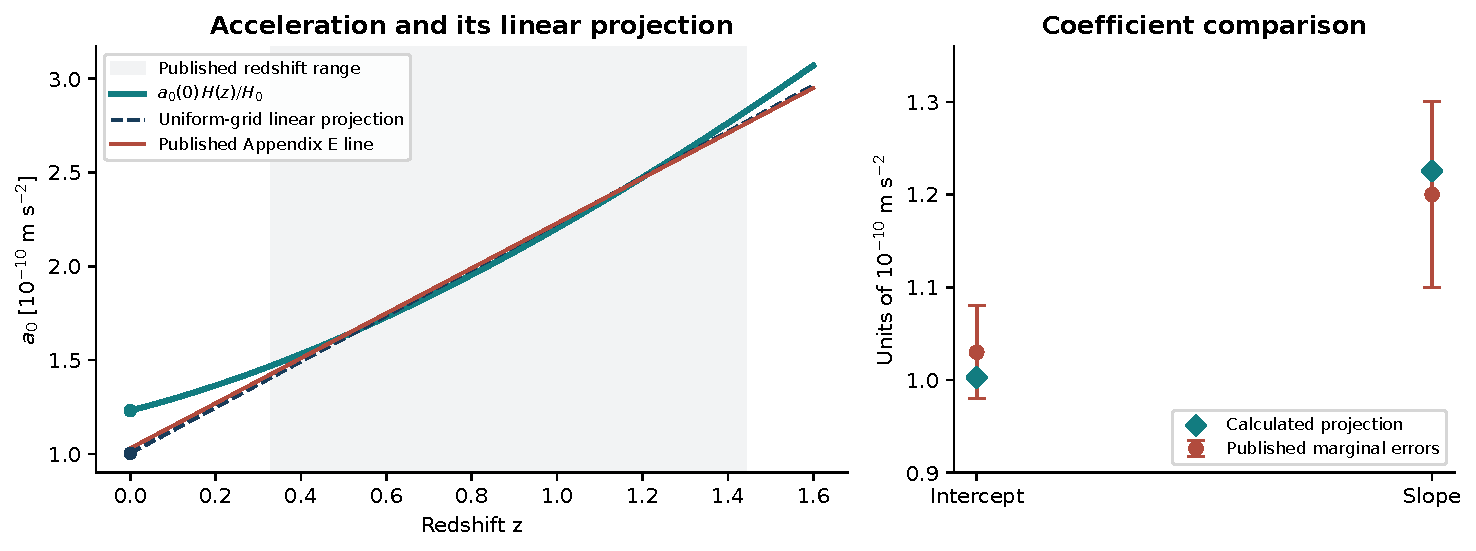
\includegraphics[width=\textwidth]{figures/redshift.pdf}
\caption{The calculated acceleration curve and its linear projection.
The published line summarizes the Appendix E inference. The right panel
shows marginal coefficient errors, with no assumption of independence.
The uniform-grid projection is not a refit to the original galaxy data.}
\end{figure}

The individual coefficient differences are $-0.54$ and $+0.26$ times the
quoted marginal errors. A joint significance requires the fitted
intercept--slope covariance and the survey's effective redshift weighting.
The two agreements are consequences of one curve, not independent
probabilities to multiply.

\subsection{A joint cosmological test}

The prediction fixes the absolute function, including normalization and
curvature. This comparison uses $\Omega_m=0.315$ and
$\Omega_\Lambda=0.685$. A joint test must use the release model's
fitted $H(z)$ in equation~\eqref{eq:a0}, propagate its uncertainty, and
fit the individual galaxies with their correlated baryonic and kinematic
errors. Galaxy formation can also produce an evolving RAR in conventional
halo models, so evolution alone does not distinguish the mechanisms.

\subsection{Catalogue tests and the direction of a relaxation correction}
The common cosmology was propagated to 73 KMOS3D, 21 KGES, and 169 KROSS
objects at three radii. At the KMOS3D outer radius, the log-acceleration
residual slope is $-0.245$ dex per unit redshift with constant $a_0$ and
$-0.313$ with the common $H(z)$ law. The latter has median log-velocity
residual $-0.087$ dex. The reference $z=2.3$ example gives acceleration
boosts about 2.02 versus 1.39 for the compared evolving and fixed scales.
These are catalogue central-value diagnostics with specified baryon force
models; they do not constitute raw-cube likelihoods. The 112-point
reference projection remains distinct from a regression on the actual
79-object MUSE selection. The common cosmology has not removed the
high-redshift residual trend. \source{U1, S01}

Passive relaxation cannot automatically supply a reduction. If
$\dot n=\Gamma(q-n)$ with $\Gamma>0$, $\dot q\le0$, and initially
$n\ge q$, then $n$ remains above the target. At fixed baryons a lag behind
declining $H$ therefore has the wrong sign to suppress an initially
equilibrated response. Underoccupied assembly states require their own
history. Relabeling an unchanged stock leaves its total stress unchanged;
the tested adiabatic cosmological mass loss gives an inferred scale ratio
0.9183 from $z=2.3$, compared with $H_0/H(2.3)=0.2972$.
These constraints identify the contact and preparation history as physical
requirements. \source{D1}

For the selected two-pole quantum response, the noise enhancement
$\mathcal F$ and mean delay $\bar\tau$ obey
$\mathcal F H\bar\tau\ge4$. The illustrative three-percent tracking
condition at occupation argument $x=1$ gives $\mathcal F\gtrsim158$,
requiring about $6.47\times10^4$ independent cells for three-percent
force rms. Actual windows, correlations, and gravitational coupling
remain unspecified, so this is a contact-model constraint.
\source{D1; T1, N.8}

\subsection{Stock selection reaches the response law}
\label{sec:stockselection}
The response law is an equilibrium of the retained stock. The stock
reaches it through a selection with three ingredients:
\begin{itemize}
\item \textbf{Occupation.} The response cell's occupation is the stock
field in baryonic units, $n=g_R/g_b$.
\item \textbf{Free energy.} Its excess free energy is the Bose relative
entropy $D(n\Vert n_*)$. Its weight is fixed by equipartition with the
excess field, $\mathcal N\Theta=g_b^2n_*(1+n_*)/4\pi G$.
\item \textbf{Contacts.} Momentum-conserving stock contacts proceed when
they lower the orbit-averaged free energy, which is the zero-temperature
limit of detailed balance with the horizon bath.
\end{itemize}
A coupling that held the stock at the response density would pass the
stock's kinematic mismatch $d$ to the baryons as a force error $-dJ'(g_b)$,
with $J'\simeq5$ at 100\,kpc. The stock therefore supports itself, and the
selection acts slowly. \source{T1, O.3; G8, G9}

Spherical three-dimensional runs use abundance-matched NFW stock with an
equilibrium Eddington distribution \cite{dutton,moster}, static
spherical-equivalent baryons, and one to three contact proposals per
orbit. They run for 12\,Gyr. Offsets from the response law are rms over
5--200\,kpc, and over 5--100\,kpc for dwarfs:
\begin{center}
\small
\begin{tabularx}{\textwidth}{lccX}
\toprule
Model & no contacts & 8--12\,Gyr & note\\
\midrule
Milky Way, 4 runs & 0.10 & 0.009--0.032 & mismatch falls to the shot-noise level\\
Dwarf, 3 seeds & 0.13 & 0.02--0.04 & 5--10\% above the exact constrained minimum\\
Massive spiral, $6\times10^{12}\Msun$ & 0.03 & 0.007--0.043 & \\
Massive spiral, $2.5\times10^{12}\Msun$ & 0.14 & 0.05 & stock budget binds; still converging\\
Full Bose functional, MW & & 0.019--0.024 & matches its Gaussian limit\\
Full Bose functional, dwarf & & 0.025--0.030 & matches its Gaussian limit\\
\bottomrule
\end{tabularx}
\end{center}
Contacts conserve momentum and angular momentum to roundoff, and the
energy ledger closes to $10^{-3}V_f^2$. The stock gains about $0.15V_f^2$
per unit mass from the work register. The mismatch decreases overall,
with fluctuations at the particle shot-noise level.

\begin{figure}[H]
\centering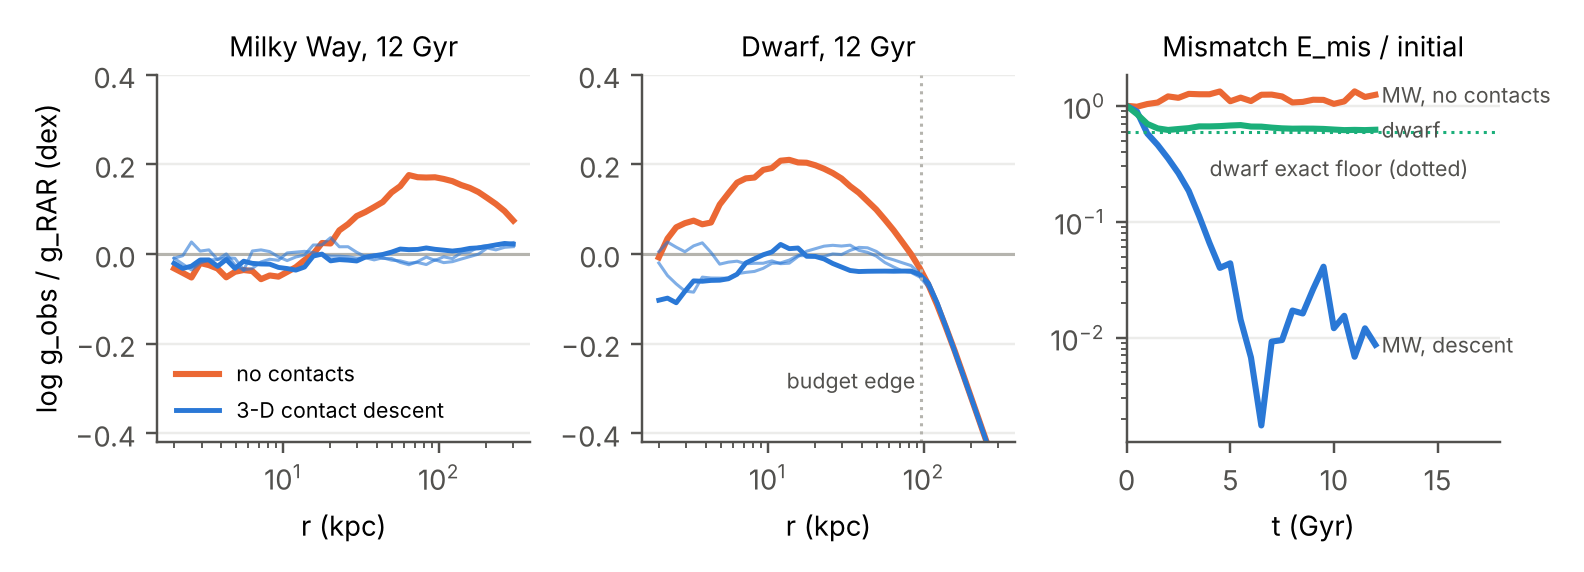
\includegraphics[width=\textwidth]{figures/stock_selection.png}
\caption{Offset from the response law after 12\,Gyr without contacts
(orange) and with contact selection (blue, three runs per model). Right:
the mismatch functional relative to its initial value; the dotted line is
the dwarf's exact constrained minimum.}
\end{figure}

\textbf{The cohort ratio inside galaxies.} Inside radius $r$ the selected
stock-to-baryon ratio equals the occupation $n_*(x)$, which rises
outward. A Milky Way model has about 0.8 inside 10\,kpc, 5.2 at 50\,kpc,
11 at 100\,kpc and 22 at 200\,kpc, up to the budget edge, where the
retained stock is exhausted. A galaxy that has lost most of its ancestral
baryons from the counted region therefore shows a total of about 30 stock
masses per present baryonic mass. The same stock, measured against the
cohort's original baryons, holds the ratio $k_C$.

\textbf{Weak lensing.} An isolated finite stock bounds the excess surface
density by $(1+S)g_{\rm bar}/\pi G$. A signal on the deep response law then
requires $S\ge\tfrac\pi4\sqrt{a_0/g_{\rm bar}}-1$: about 12 at
$4.7\times10^{-13}$, 31 at $7.6\times10^{-14}$ and 275 at
$10^{-15}\,\mathrm{m\,s^{-2}}$. Stocks of about 30 fit the inner KiDS
bins \cite{brouwer21}. The carried stock ends with the support, where
hot gas outweighs the condensed baryons, and the uncarried stock outside
keeps the halo profile. A population forward model of the four isolated
stellar-mass bins of \cite{brouwer21}, with 60 points, full covariance,
the same hot gas and a common environment term, gives $\chi^2=140$ for
the support-limited stock against $133$ for truncated NFW halos when
both fit a halo-mass shift and a concentration factor. Both leave
$3$--$6\sigma$ residuals at $0.5$--$1.5\,$Mpc, where neighbouring
structure contributes. \source{G8, G12}


\section{The LMC and inherited gravitating stock}
\label{sec:lmc}

For $3\times10^9\Msun$ of LMC baryons, the retained-stock prescription gives
\begin{equation}
M(<30\,\mathrm{kpc})=5.0348\times10^{10}\Msun,
\qquad
M(<50\,\mathrm{kpc})=8.2896\times10^{10}\Msun.
\label{eq:lmcmasses}
\end{equation}
Warren et al. infer $(4.7$--$5.1)\times10^{10}\Msun$ inside 30 kpc from
the Orphan--Chenab stream. Brooks et al. infer
$8.76^{+1.94}_{-1.77}\times10^{10}\Msun$ inside 50 kpc from outer-halo
kinematics. The calculated masses agree with both quoted results.
\cite{warren,brooks}

In the same baryonic configuration, the tested QUMOND external-field
calculations give only $(1.54$--$1.68)\times10^{10}\Msun$ of effective
enclosed LMC mass inside 30 kpc. The difference comes from whether the
system retains its previously established stock when it enters the Milky
Way environment. \source{G1, G2}

\subsection{From an acceleration law to an enclosed mass}

Outside most of the LMC's baryons, use the spherical point-source
approximation
\begin{equation}
g_b(r)=\frac{GM_b}{r^2},\qquad
r_M=\sqrt{\frac{GM_b}{a_0}}.
\end{equation}
Equation~\eqref{eq:rar} then gives
\begin{equation}
g_{\rm obs}(r)=\frac{GM_b}{r^2[1-e^{-r_M/r}]}.
\end{equation}
The effective enclosed mass is defined through $g_{\rm obs}=GM(<r)/r^2$,
so
\begin{equation}
M(<r)=\frac{M_b}{1-e^{-r_M/r}},\qquad
M_R(<r)=M(<r)-M_b.
\label{eq:lmcprofile}
\end{equation}
The baryonic term and the extra stock are counted once each.

With $G=4.30091\times10^{-6}\,\mathrm{kpc}\,(\mathrm{km/s})^2\Msun^{-1}$,
$a_0=3798.47\,(\mathrm{km/s})^2\mathrm{kpc}^{-1}$, and the stated baryonic
mass, $r_M=1.84305\,\mathrm{kpc}$. At 30 kpc the exponent is
$r_M/r=0.061435$, and
\begin{equation}
M(<30)=\frac{3\times10^9}{1-e^{-0.061435}}\Msun
=5.0348\times10^{10}\Msun.
\end{equation}
At 50 kpc the exponent is $0.036861$, giving the second mass in
equation~\eqref{eq:lmcmasses}. A Plummer baryonic profile with scale
$1.5\,\mathrm{kpc}$ changes these outer values only slightly.

In the deep regime,
\begin{equation}
M(<r)=\sqrt{\frac{M_ba_0}{G}}\,r+\frac{M_b}{2}
+O(r_M/r).
\end{equation}
The enclosed mass grows approximately linearly with radius, giving an
approximately flat circular speed before the finite stock budget limits
the profile. This also shows the main sensitivity:
$M(<r)\propto M_b^{1/2}a_0^{1/2}r$. A fractional baryonic-mass error
contributes about half as much fractional mass error at these radii.
The central numbers do not imply negligible uncertainty in the baryons.

\subsection{Why the budget refers to ancestral baryons}

The initial commitment is bounded by $M_{b,L}/\epsilon$, where $M_{b,L}$
is the baryonic content of the Lagrangian source whose history is followed.
In the linear-depletion benchmark used for the saved galaxy calculations,
a full release removes the share $\eta_*$. Its carrier budget is
\begin{equation}
M_R\le \frac{1-\eta_*}{\epsilon}M_{b,L},\qquad
C_R\equiv\frac{M_{R,\max}}{M_{b,\rm present}}.
\label{eq:cap}
\end{equation}
Loss of gas or redistribution of baryons can make $C_R$ much larger than
$1/\epsilon$. A large present stock-to-star ratio is compatible with a
finite initial commitment per ancestral baryon.

Writing $M_{b,L}=f_bM_h$ gives the manuscript's useful parameterization
\begin{equation}
C_R\simeq(1-\eta_*)(1-f_b)\frac{M_h}{M_{b,\rm present}},
\end{equation}
when $f_b/(1-f_b)\simeq\epsilon$. Here $M_h$ identifies the ancestral
assembly mass used for the budget. It is an astrophysical history input.
Its use does not follow from the cell count alone.

The numerical LMC model uses $C_R=33$, so the total mass cap is
$(1+C_R)M_b=1.02\times10^{11}\Msun$. Equation~\eqref{eq:lmcprofile} reaches
that cap at
\begin{equation}
r_{\rm cap}=-\frac{r_M}{\ln[1-(1+C_R)^{-1}]}=61.74\,\mathrm{kpc}.
\end{equation}
The quoted 30 and 50 kpc predictions lie inside the cap. Their values
are insensitive to its exact location. The composition-preserving
allocation replaces $1-\eta_*$ by $e^{-\eta_*}$ for complete ensemble
release, increasing this budget by $0.0455\%$. The reported masses and
satellite trajectories retain their original benchmark convention. \source{T1, O.3; G1}

\subsection{Persistence, transport, and tidal stripping}

Retained stock has a positive density and an advected mass. A collisionless
description uses a phase-space distribution $f_R(\mathbf x,\mathbf v,t)$
obeying
\begin{equation}
\frac{\partial f_R}{\partial t}
+\mathbf v\cdot\nabla_x f_R
-\nabla\Phi\cdot\nabla_v f_R=0,
\qquad
\rho_R=\int f_R\,d^3v,
\label{eq:vlasov}
\end{equation}
between formation, release, and carrier-reorganization events. Integrating
over velocity gives a continuity equation for $\rho_R$. A change in the
host's gravitational field can move the stock, distort it, or remove some
of it from the satellite. It does not algebraically erase its mass.

A spatially uniform external acceleration mainly accelerates the carrier
as a whole. Tides arise from the field gradient, represented locally by
$\partial_i\partial_j\Phi_{\rm host}$. They can unbind the extended stock
because its outer orbits are weakly bound. This is the physical difference
between losing stock through transport and reducing a static effective
gravity law because the external field changed.

The theory's equilibrium contact and its persistent-stock dynamics are
different stages of the same proposed mechanism. The contact specifies a
target profile for a coherent carrier; collisionless evolution follows
that profile after infall. The manuscript also allows mass-conserving
relaxation toward carrier-resolved equilibrium. The available satellite
runs use retained stock with no subsequent contact relaxation. Its rate
and its derivation from the native microscopic dynamics remain to be fixed.

\subsection{The external-field comparison}

In QUMOND, the field equation contains the nonlinear flux
$\nu(|\mathbf g_N|/a_0)\mathbf g_N$, where the Newtonian field includes
both host and satellite. The local calculation estimates the LMC's
equivalent enclosed mass by subtracting the host-only flux:
\begin{align}
M_{\rm LMC}^{Q}(<r)=-\frac1{4\pi G}\oint_{S_r}
\Big[&\nu\!\left(\frac{|\mathbf g_{N,L}+\mathbf g_{N,MW}|}{a_0}\right)
(\mathbf g_{N,L}+\mathbf g_{N,MW})\nonumber\\
&-\nu\!\left(\frac{|\mathbf g_{N,MW}|}{a_0}\right)
\mathbf g_{N,MW}\Big]\cdot d\mathbf A.
\label{eq:flux}
\end{align}
This is an effective gravitational mass, not a count of extra matter
particles. The host subtraction matters because the flux is nonlinear.

The computation uses a $10^{10}\Msun$ Hernquist bulge, a
$5\times10^{10}\Msun$ Miyamoto--Nagai disk, a $3\times10^9\Msun$
Plummer LMC, and a 50 kpc separation. Direct angular quadrature uses
96 Gauss--Legendre points and 192 azimuthal points. Re-execution gives
\begin{center}
\begin{tabular}{lc}
\toprule
Response prescription & $M(<30\,\mathrm{kpc})/[10^{10}\Msun]$\\
\midrule
Retained spherical stock & 5.035\\
QUMOND, exponential RAR function & 1.679\\
QUMOND, simple function & 1.681\\
QUMOND, standard function & 1.539\\
\bottomrule
\end{tabular}
\end{center}
The tested external-field models fall a factor of roughly three below the
cited 30 kpc inference. The difference persists across these three
interpolation choices. A complete comparison would evolve the observed
stream in each time-dependent model and compare its positions and
velocities directly. The published mass posterior was inferred using
gravitational models; it is not a raw model-free datum.

\begin{figure}[htbp]
\centering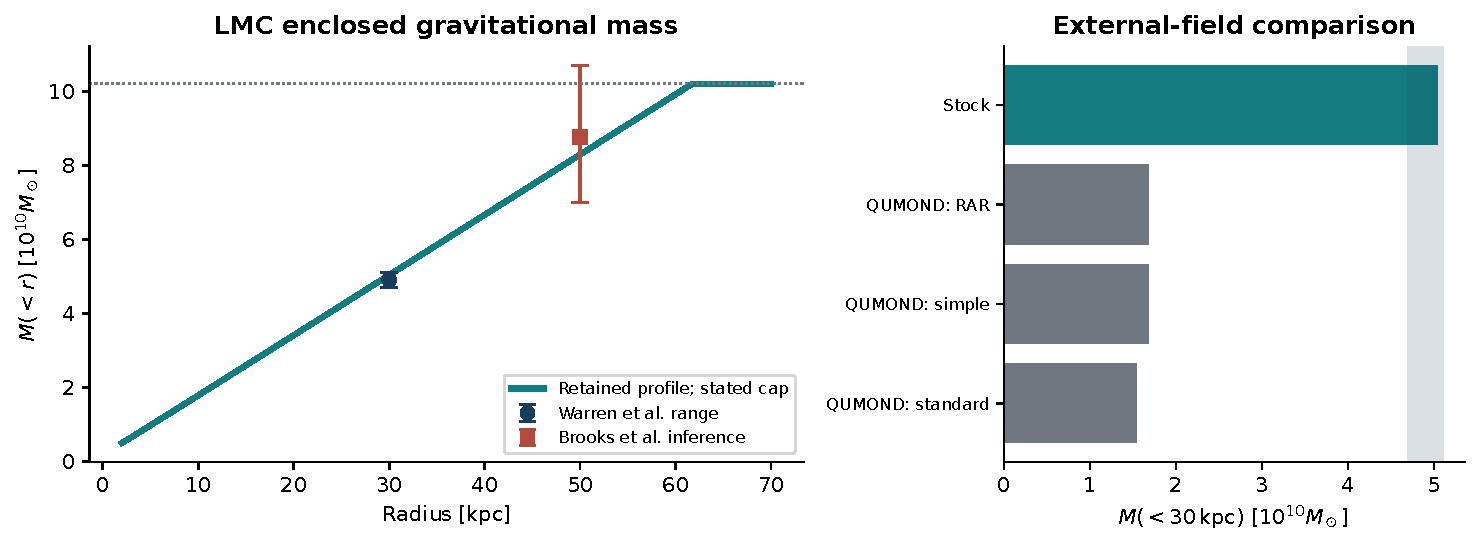
\includegraphics[width=\textwidth]{figures/lmc.pdf}
\caption{The retained LMC mass profile, its finite budget, and the
recomputed QUMOND flux comparison. The 30 kpc bar represents the reported
range of stream inferences, not a Gaussian one-sigma interval. The 50 kpc
bar uses the published asymmetric uncertainties.}
\end{figure}

\subsection{The reflex motion tests inertia}

An extended gravitating component should also accelerate the Milky Way.
Brooks et al. infer a reflex speed
$38.6^{+8.3}_{-7.8}\,\kms$ relative to halo stars at 100 kpc, jointly
with the LMC and Milky Way masses. That observable tests the dynamical
interaction, including the response of the outer halo. \cite{brooks}

The available moving-LMC calculation produces a Milky Way acceleration
corresponding to about $35\,\kms$ over the last gigayear. This establishes
the relevant scale. A direct comparison requires the same halo reference
population, spatial selection, and velocity estimator as the observation.
The present calculation also uses the usual asymmetric pair-force
approximation, while the theory requires reciprocal forces from its joint
source action. These distinctions prevent a precise reflex likelihood
claim from being assigned to the saved run. \source{G4}

The physical implication of a successful reflex calculation would be
strong: the extra gravity would participate in the momentum balance of
the system. Agreement of an isolated rotation curve alone cannot establish
that property.

\subsection{Tidal dwarfs test which source owns the response}

A tidal dwarf forms from material pulled out of a larger galaxy. Its gas
and stars already belong to an ancestral source. The carrier rule assigns
them to that inherited record while the parent remains dynamically
coherent. Applying a new isolated equilibrium law to the dwarf's own
baryons would count a new independent response at the wrong stage of its
history.

Exact projectors act on disjoint active record labels. Smooth spatial
weights used to distribute an effective source form a separate partition
of unity; they carry no projector-idempotence requirement. If $P$
is the active parent, its descendants contribute to the parent source
before the nonlinear response is evaluated. Parent and child are not
simultaneously counted as independent sources of an extra halo. A
descendant in the parent's retained response also inherits its director,
the orientation field that controls the transverse flux.
\source{T1, section 15 and N.8}

The director's stiffness controls its response to a local tilt of the
source. In the linearized description, a mode of wavenumber $k$ has
transfer factor
\begin{equation}
\frac{\delta\boldsymbol n(k)}{\delta\boldsymbol n_{\rm eq}(k)}
=\frac{1}{1+k^2\xi^2},
\end{equation}
where $\xi$ is the director coherence length fixed by the effective
stiffness. A descendant samples the parent's coherent director. A
separate carrier has its own stiffness and director. The inherited
orientation suppresses the local transverse response that the
independent-carrier calculation would allow. \source{G5}

The numerical proxy converts each resulting force field into a virial
dispersion. For a stationary tracer distribution of mass $M$, define
\begin{equation}
W=-\int\rho(\boldsymbol r)\,
\boldsymbol r\cdot\boldsymbol\nabla\Phi\,d^3r.
\end{equation}
The scalar virial relation $2K+W=0$ gives the direction-averaged
one-dimensional dispersion $\sigma^2=-W/(3M)$, and hence the boost
$\sigma^2/\sigma_N^2=W/W_N$. The force calculation, inherited orientation,
and tracer profile determine this ratio. The observed gas rotation still
requires a separate geometrical and dynamical interpretation.

The available NGC 5291 comparison uses three dynamical-to-baryonic mass
ratios, $1.5\pm0.7$, $1.3\pm0.5$, and $1.2\pm0.7$, and a parent of
$2\times10^{11}\Msun$ at 60 kpc. The inherited response gives modest
enhancements. Treating the dwarfs as separate isolated carriers gives
much larger enhancements. \source{G1, G5}\cite{lelli}
\begin{center}
\begin{tabular}{lcc}
\toprule
Prescription & Mass enhancement & Reported $\chi^2$ for three objects\\
\midrule
Parent-carrier inheritance & 1.5--2.0 & 0.5\\
Separate isolated carriers & 3.6--4.9 & 48\\
Newtonian baryons & 1.0 & 1.0\\
\bottomrule
\end{tabular}
\end{center}
The calculation uses a virial-response proxy, with the enhancement read
through $\sigma^2/\sigma_N^2$. It does not supply a resolved,
non-equilibrium gas-dynamical fit to every dwarf. Its evidential force is
the rejection of the separate-carrier prescription within this test.
Newtonian baryons also fit these ratios, so these three objects do not
uniquely select the capacity model or exclude conventional tidal dwarfs.

\section{Cold dwarf remnants and tidal inheritance}
\label{sec:crater}

Crater II combines a large projected half-light radius with a small stellar
velocity dispersion. The moving-Milky-Way-plus-LMC calculation produces a
surviving stock remnant with
\begin{equation}
\sigma_{\rm los}=2.36\,\kms,\quad R_h=0.86\,\mathrm{kpc},\quad
M_*=3.2\times10^5\Msun,\quad f_{\rm tail}=0.23.
\label{eq:craterbest}
\end{equation}
A second well-ranked state gives
$(2.18\,\kms,1.24\,\mathrm{kpc},4.4\times10^5\Msun,0.38)$.
The comparison data used by the likelihood are
$(2.7\pm0.3\,\kms,1.066\pm0.084\,\mathrm{kpc},
3.2\pm1.0\times10^5\Msun,0.23\pm0.08)$.
The first state matches the dispersion, mass, and adopted tail statistic
well, while its radius is about 19\% low. The second is larger and has
more stellar debris. \source{G3, G4}

Against the specified NFW halo ensemble, the moving-LMC comparison gives
$B=1.98\times10^8$ for 0.3-dex halo-mass scatter and
$B=2.62\times10^5$ for 0.5-dex scatter when the fractional model error is
10\%. These values have been recomputed from the saved run outputs for
this document. They quantify a preference for the stock construction
within this numerical experiment.

\subsection{Which satellites keep their stock}

A satellite has its own cells only where its own baryonic field exceeds
the host's. At the three-dimensional half-light radius the ratio of the
Milky-Way law field to the dwarf's own law field is $5.5$ for Sextans,
$2.5$ for Draco, $2.0$ for Ursa Minor and $1.7$ for Carina, which keep
their pre-infall stock, and $0.98$ for Sculptor, $0.38$ for Fornax,
$0.20$ for Leo~II and $0.09$ for Leo~I, which relax. Scored on the
GravSphere central densities $\rho(150\,{\rm pc})$ \cite{read19}, this
assignment gives $\chi^2=10.4$ over the eight dwarfs, against $17.2$
for retained stock throughout and $44$ for relaxed stock throughout.
Ten of the $256$ retained or relaxed assignments reach
$\chi^2\le10.4$; the best, $5.7$, also retains Leo~II. The
classification holds for Milky-Way baryonic masses of
$5$--$6\times10^{10}M_\odot$, cap ratios of $10$--$20$, projected or
three-dimensional radii, and Newtonian or law fields, with Sculptor on
the boundary. \source{G12}

A dwarf whose main progenitor never crossed the release gate of
Section~\ref{sec:cosmology} keeps its committed allocation, and its stock
stays collisionless. Over 22 Local Group dwarfs with half-light masses
from the Local Volume Database, relaxed masses from contact runs, and gate
crossing from the mean accretion history of Fakhouri et al. (2010), this
combined assignment gives $\chi^2=21.7$ at the reference gate of
$17\,\kms$ and $25.4$ at $14\,\kms$. \LCDM\ halos with supernova heating
at the published coreNFW calibration give $24.0$, and NFW halos without
heating give $30.0$. Over plausible accretion histories, M31 baryonic
masses and the two published Tucana dispersions, the combined assignment
spans $18.5$--$29.2$ and heating spans $23$--$25.5$; these data do not fix
the gate. \source{G12}

\subsection{Why size and dispersion must be explained together}

In a dispersion-supported system, random stellar velocities provide
support against gravity. Under equilibrium and approximate spherical
symmetry, a useful scale estimate is
\begin{equation}
M(<r_{1/2})\simeq\frac{3r_{1/2}\sigma_{\rm los}^2}{G}
\simeq\frac{4R_h\sigma_{\rm los}^2}{G},
\label{eq:wolf}
\end{equation}
where $r_{1/2}\simeq4R_h/3$ is the three-dimensional half-light radius.
For the adopted Crater II values this gives roughly
$7.2\times10^6\Msun$. The estimate is a guide to the required depth of
the central potential; a tidally disturbed galaxy requires direct
modeling. \cite{wolf}

Reducing a halo's central mass can cool the stars, but its tidal response
can also contract or destroy the stellar distribution. A successful model
must retain a diffuse body while reducing its binding potential, and
must leave the right amount of visible debris. A dispersion fit at an
incorrect radius addresses only part of the problem.

\subsection{Initial conditions and the physical stock profile}

The stellar progenitor is a Plummer sphere,
\begin{align}
\rho_*(r)&=\frac{3M_*}{4\pi b^3}
\left(1+\frac{r^2}{b^2}\right)^{-5/2},\\
M_*(<r)&=M_*\frac{r^3}{(r^2+b^2)^{3/2}}.
\end{align}
Its projected half-light radius is $b$. The progenitor's isolated stock is
initialized from
\begin{equation}
M_R(<r)=\min\left\{M_*(<r)
\left[\nu\!\left(\frac{GM_*(<r)}{a_0r^2}\right)-1\right],
C_RM_*\right\},
\label{eq:dwarfstock}
\end{equation}
with $\nu(y)=(1-e^{-\sqrt y})^{-1}$ and $C_R=3000$.
The differentiated density is tapered by $e^{-(r/12\,\mathrm{kpc})^2}$.
The cap and taper are specified modeling inputs tied to the proposed
history and its numerical realization. They are not independently
measured halo properties of Crater II.

The central form explains why stock responds differently from a cusp.
For $r\ll b$, the Plummer mass scales as $r^3$, so $g_b\propto r$.
In the low-acceleration limit, $\nu-1\propto r^{-1/2}$. Consequently
\begin{equation}
M_R(<r)\propto r^{5/2},\qquad \rho_R(r)\propto r^{-1/2}.
\end{equation}
This is shallower than the $r^{-1}$ inner density of an NFW halo. The
outer stock is extended and weakly bound. Tides can remove substantial
stock and lower the stellar velocity scale without forcing the same
stellar contraction as in the tested NFW models.

Both stars and stock are initialized through isotropic Eddington
distribution functions in the combined potential. This matters because
the initial density profile alone does not specify stellar velocities.
For relative potential $\Psi=-\Phi+\Phi(\infty)$ and relative energy
$\mathcal E=\Psi-v^2/2$, the inversion can be written
\begin{equation}
f(\mathcal E)=\frac{1}{\sqrt8\,\pi^2}\frac{d}{d\mathcal E}
\int_0^{\mathcal E}\frac{d\rho/d\Psi}{\sqrt{\mathcal E-\Psi}}\,d\Psi.
\end{equation}
At a sampled radius, speeds are drawn with probability proportional to
$v^2f(\Psi-v^2/2)$. The code evaluates the inversion on a finite radial
grid and clips negative numerical values of $f$ to zero; equilibrium and
resolution controls are needed to assess this approximation.
Equilibrium phase-space sampling avoids using an arbitrary initial
velocity dispersion as a hidden fit parameter. \source{G1, G3}

\subsection{The orbit and the LMC perturbation}

The calculation uses the present position, distance, radial velocity, and
proper motion to infer a past orbit in each gravitational model. The
adopted Crater II inputs are $D=117.5\,\mathrm{kpc}$,
$v_{\rm los}=87.5\,\kms$, and
$(\mu_{\alpha*},\mu_\delta)=(-0.07,-0.11)\,\mathrm{mas\,yr^{-1}}$.
The stock Milky Way contains $6\times10^{10}\Msun$ of baryons and a
retained profile with $C_R=14$.

The moving LMC carries $3\times10^9\Msun$ of Plummer baryons and its
retained profile, capped at $1.02\times10^{11}\Msun$ in total.
The trajectory includes a specified Chandrasekhar friction term and
the acceleration of the Milky Way. In this calculation Crater II's latest
pericentre is 25.3 kpc, 1.68 Gyr before the present, in the stock host;
the NFW comparison gives 24.9 kpc. The models use the same observed
phase-space inputs, but their host potentials give distinct orbits.
\source{G4}

Only first-pericentre stock progenitors survive in the sampled moving-LMC
grid. Its best state begins with twice today's stellar mass and
$0.7R_{h,\rm obs}$. The next state begins with four times today's mass
and $R_{h,\rm obs}$. The agreement includes inference over progenitor
mass, size, and infall age within a prior-weighted grid.

A rough tidal-radius estimate makes the mechanism clear. For a small
satellite on a circular orbit of radius $R$ in a spherical host,
\begin{equation}
r_t\simeq R\left[
\frac{m(<r_t)}{[3-d\ln M_H/d\ln R]M_H(<R)}
\right]^{1/3}.
\end{equation}
The real orbit is eccentric and the LMC makes the potential time
dependent, so the simulation integrates the forces directly. Near
pericentre, the strongest differential field removes the weakly bound
outer stock. The retained stellar body then responds to a shallower
potential. Its final dispersion is an output of this evolution.

\subsection{What the numerical experiment actually resolves}

The shared solver follows 40,000 stock or dark particles and 10,000 stellar
particles with a one-Myr leapfrog step and 0.03 kpc softening. Self-gravity
is computed through a monopole about the density centre. The external
Milky Way and LMC fields are applied to the particles. This is a
collisionless particle experiment with spherical internal force
resolution, not a full unrestricted tree-gravity calculation.

The comparison uses NFW subhalos with a Moster stellar-to-halo mass prior
and the Dutton--Macci\`o median concentration relation. Progenitor masses
are one, two, or four times today's stellar mass; sizes are $0.7$, $1.0$,
or $1.5$ times the observed half-light radius, weighted by the stated
size--mass prior. The infall-age grid counts pericentric passages.
The enlarged halo grid includes masses far below the central
abundance-matching expectation. \source{G3, G4}\cite{moster,dutton}

The NFW models approach the observed dispersion at inferred infall masses
around $10^{7.4}$--$10^{7.7}\Msun$, about two dex below the reference
abundance-matching relation. Their radii then lie near 0.76--0.78 kpc and
their dispersions near 3.2--3.5 $\kms$. The two-dex statement describes
the required prior displacement in this model family. It is not a universal
proof that a galaxy could never have formed in such an object: gas
retention, early cooling, concentration, and assembly history also matter.

\subsection{Tail counts and the measurement procedure}

The MAGIC photometric sample contains 162 candidate red-giant members,
37 of them in the tails, giving $37/162=0.2284$. The reported stream width
is about $0.8^\circ$, and the tails extend beyond the observed footprint.
These are population- and selection-dependent measurements. A candidate
count is not automatically a complete fraction of all stellar mass.
\cite{atzberger}

The grid likelihood uses $f_{\rm tail}=0.23\pm0.08$ and a statistic counting
stars beyond $3R_{h,\rm obs}$ within a three-dimensional radius of about
14.4 kpc. The central dispersion is measured from bound stars within
$1.5R_h$ in projection. These definitions can be reproduced from the
simulation, but the observing program does not have direct access to a
bound-particle label or a spherical three-dimensional membership cut.
A final comparison needs the photometric footprint, candidate selection,
velocity errors, gradient subtraction, and foreground model applied to
mock observations.

Independent spectroscopy now confirms cold central kinematics and
provides a stream-to-body dispersion ratio. Limberg et al. report
$2.51^{+0.33}_{-0.30}\,\kms$ for the body and
$5.74^{+0.98}_{-0.83}\,\kms$ for the stream. Their own simulations find
the dispersion ratio difficult for standard-concentration cusps, while
cored or low-concentration halos can reproduce it. The stock model should
predict this ratio and the stream width as additional observables.
\cite{limberg}

\subsection{The strength and the scope of the model comparison}

For an observable $O_j$, the grid uses an effective error
$s_j^2=\sigma_{j,\rm obs}^2+(f_{\rm mod}O_{j,\rm model})^2$ for
dispersion and radius. Its Gaussian likelihood includes the $1/s_j$
normalization. With fixed observational errors for stellar mass and
tail fraction,
\begin{equation}
\mathcal L(\theta)\propto
\prod_j\frac1{s_j}
\exp\left[-\frac{(O_{j,\rm model}(\theta)-O_{j,\rm obs})^2}{2s_j^2}\right].
\end{equation}
Destroyed states receive zero likelihood. The evidence is a discrete
prior average, $Z=\sum_iw_i\mathcal L_i/\sum_iw_i$ for the normalized
grid, with the documented Gaussian mass-prior quadrature for the extended
halo tail. The Bayes factor is $B=Z_{\rm stock}/Z_{\rm NFW}$.

\begin{center}
\small
\begin{tabular}{lrr}
\toprule
Fractional model error & With LMC, 0.3-dex mass scatter & With LMC, 0.5 dex\\
\midrule
10\% & $1.98\times10^8$ & $2.62\times10^5$\\
20\% & $2.99\times10^3$ & $9.26\times10^2$\\
30\% & $1.55\times10^2$ & $9.42\times10^1$\\
\bottomrule
\end{tabular}
\end{center}

The preference remains in the same direction throughout these sensitivity
checks, while its numerical magnitude changes by several orders of
magnitude. The quoted large factors require the 10\% model-error assumption. The
numerical errors, force approximation, orbit uncertainty, and observation
mapping should determine that error budget independently.

\begin{figure}[htbp]
\centering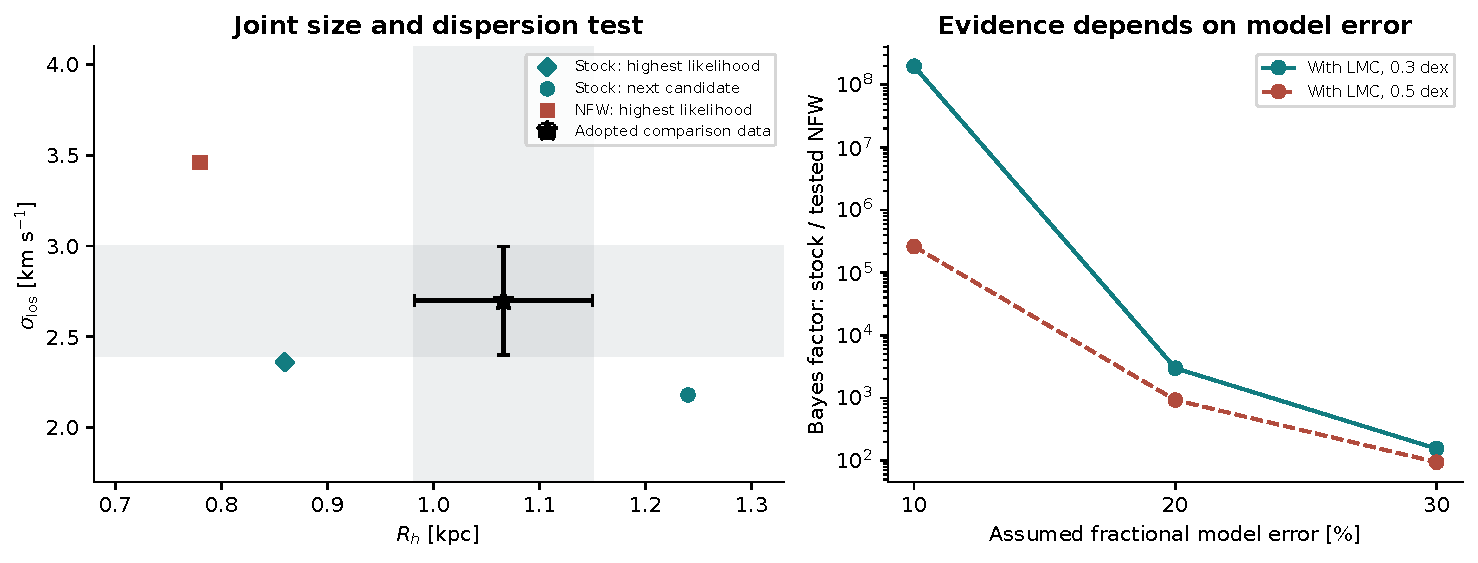
\includegraphics[width=\textwidth]{figures/crater.pdf}
\caption{The moving-LMC Crater II comparison and its dependence on the
assumed model error. The left panel emphasizes the joint size and
dispersion constraint. The evidence calculation also uses stellar mass
and the adopted tail fraction. The two halo priors use the same saved
particle trajectories.}
\end{figure}

The archived record describes a hash-locked core protocol preceding the
comparison campaign. The moving-LMC extension and enlarged mass priors
are documented follow-ups.
The present file hash matches the stored registration hash. A matching
hash verifies file identity; by itself it does not independently certify
the historical ordering of executions. \source{G3, G4, G6}

The tested alternative consists of cuspy halos at a prescribed
concentration relation. It does not cover the full range of concentration
scatter, feedback-induced cores, or every dark-matter model. Crater II
therefore favors the stock model strongly over this specified alternative.
It does not establish odds against the entire \LCDM\ framework.

The moving-LMC satellite grid was reweighted with ten, twenty, and
thirty percent model uncertainty. At thirty percent the Crater II
stock/NFW evidence falls to 94--155 from $2.6\times10^5$--$2.0\times10^8$
at ten percent; Antlia 2 rises from 0.007--0.019 to 0.69--0.74.
The grid does not implement the new conservative joint-stock contact
or span broad cored-halo alternatives. Its evidence remains conditional
on the specified histories, priors, and error budget. \source{U1, S14}

\subsection{Antlia 2: a recently disturbed system still requires a successful mock observation}

Antlia 2 has a measured dispersion
$5.98^{+0.37}_{-0.36}\,\kms$ after fitting a velocity gradient.
The gradient is $5.72^{+0.60}_{-0.56}\,\kms$ per degree. Ji et al. find
evidence of tidal disturbance and show that its orbital interpretation
requires the LMC-induced reflex of the Milky Way. \cite{ji}

In the available moving-LMC stock runs, five of the 27 states survive.
The best bound remnant has $\sigma=3.48\,\kms$,
$R_h=2.41\,\mathrm{kpc}$, and $M_*=9.4\times10^5\Msun$.
Its most recent pericentre is about 0.79 Gyr ago. The NFW comparison can
approach the adopted observables using low-mass halos; on the original
bound-star likelihood it is favored over the stock by about 50--140.
\source{G4}

The suggestion that Antlia 2 has not had enough time to reveal a settled
internal dispersion can be made quantitative. Using its observed radius
and dispersion,
\begin{equation}
t_{\rm cross}\sim\frac{R_h}{\sigma}
\simeq0.978\,\frac{2.92}{5.98}\,\mathrm{Gyr}
\simeq0.48\,\mathrm{Gyr}.
\end{equation}
The elapsed time is only about 1.6 such crossing times; using the best
stock remnant gives a crossing time near 0.68 Gyr. A dynamically disturbed
state is plausible. This concerns time since disturbance, not the age
of its stellar population.

The available approximate mock analyses show that unbound members and
velocity-mixture choices can move the inferred dispersion substantially.
They even change the relative ranking of the tested models. That is a
reason to use the observed selection and membership procedure. A
quantitative explanation of the measured 6 $\kms$ remains to be established.
The collisionless integrations already contain the tidal evolution;
a successful non-equilibrium account must show how that evolution produces
the measured dispersion, gradient, density profile, and membership sample
together. Antlia 2 remains an unresolved test of the current construction.
\source{G6}

\subsection{What the Crater II result changes}

The successful stock trajectories show that a diffuse cold remnant can
emerge from a specified positive mass component tied to baryonic history.
This challenges the assumption that the excess gravity of such a dwarf
must be recalculated from its present stars, or must be supplied by a
standard-concentration NFW subhalo with the adopted abundance prior.
The mechanism is explicit: outer stock is stripped, the central potential
weakens, and a substantial stellar body survives.

The next discriminants are the full stream structure, the velocity
distribution including unbound stars, and an independently controlled
model-error budget. They test the same history that produced the central
dispersion, so they can constrain the model without introducing a new
halo normalization for each observable.

\section{Common coefficients and additional discriminants}
\label{sec:discriminants}

\subsection{A common CMB-to-galaxy normalization}
\label{sec:crossnorm}
The bare commitment ratio and galactic scale obey
\begin{equation}
\left(\frac{\rho_{C,i}}{\rho_{b,i}}\right)_{\rm bare}=\frac1\epsilon,\qquad
a_0(z)=\epsilon cH(z),\qquad
a_0(z)\left(\frac{\rho_{C,i}}{\rho_{b,i}}\right)_{\rm bare}=cH(z).
\end{equation}
The fitted formation convention includes the mass-conversion factor
$f_m=5.333\epsilon$, and release leaves the homogeneous survival factor
$s(z)=e^{-\eta_*F(z)}$. On the undepleted background branch, the
observable stock ratio therefore satisfies
\begin{equation}
a_0(z)\frac{\bar\rho_C(z)}{\bar\rho_b(z)}=f_m s(z)cH(z).
\label{eq:crossnorm}
\end{equation}
The standard linear-depletion configuration gives
$H_0=68.458\,\kms\,\mathrm{Mpc}^{-1}$ and
$a_0(0)=1.25005\times10^{-10}\,\mathrm{m\,s^{-2}}$,
about 1.6\% above the reference value. The exponential-allocation fit with
massless neutrinos, linear lensing and a low-redshift supernova offset gives
$H_0=68.93885586416\,\kms\,\mathrm{Mpc}^{-1}$ and
$a_0(0)=1.25883\times10^{-10}\,\mathrm{m\,s^{-2}}$,
about 2.3\% above the reference value. Each value follows from its fitted
$H_0$ without a separate fit of $a_0$.
This is a conditional relation between sectors. Cosmological abundance
and $H_0$ are inferred together; galaxy mass calibration limits the
elementary empirical comparison to roughly twenty percent. The tilt-mode
lever and mass convention retain their physical matching assumptions.
\source{U1, S02; T4--T5}

\subsection{Newton's constant and charged-lepton masses}
\label{sec:constants}
The selected particle-coefficient route gives
$G=6.6742890813\times10^{-11}\,\mathrm{m^3\,kg^{-1}\,s^{-2}}$,
$-0.073$ quoted CODATA standard deviations; the muon ratio is
$206.768280237$, at $-0.535$ quoted standard deviations. Its tau mass
is 1776.9188 MeV against $1776.93\pm0.09$ MeV. Of the 401 tested
routing integers, only the integer $7$ lies within two quoted standard deviations
for the stated route; of 43 tested Farey candidates, only $2/7$ lies
within one. These finite-menu uniqueness checks do not quantify the
historical search over possible formulas. The measured Newton scale
and marked-formula residuals were known during development.
\source{U1, S11}\cite{constantsnew}


\subsection{Halo tilt and a common Milky Way--LMC history}
\label{sec:halo}
Three eight-Gyr halo phase realizations retain late stock tilts of
$39.58^\circ$--$42.36^\circ$ and stellar tilts of
$21.38^\circ$--$22.33^\circ$. Rounding and precession persist.
These are repeatable outcomes of the specified kinetic model, with
force convergence and stationary formation still unresolved. The
aligned-branch failure remains part of the comparison. A common
Milky Way--LMC--stream fit remains open. The archived Galactic masses
inside 50 kpc exceed the cited constraint; Section~\ref{sec:jointtest}
quantifies that mismatch. \source{U1, S13; G3--G7}



\subsection{Old-disk vertical gravity}
\label{sec:olddisk}
At the exponential fit's rounded $a_0=1.2588\times10^{-10}\,\mathrm{m\,s^{-2}}$, the reduced
old-disk solver gives NGC~628 $\chi^2=2.04$ for five dispersions and
a $-0.21\sigma$ radial--vertical mass offset. The approximate algebraic
QUMOND comparison gives $\chi^2=8.95$ and $-2.91\sigma$. The small
normalization change preserves the earlier pattern. Gas-profile,
inclination, and scale-height uncertainties remain, and a round
conventional halo can give similar vertical gravity.
\source{U1, S15}


\subsection{Wide binaries and Solar-System null tests}
\label{sec:binaries}
With the parent-carrier rule, a wide binary has no independent capacity
halo. A radial Galactic-tide estimate for one to two solar masses at
10--30 kAU gives $\Delta v/v\simeq1.1\times10^{-5}$--$6\times10^{-4}$.
The range depends on separation, mass, and orientation; a universal
$10^{-4}$ ceiling is unwarranted. The selected Solar quadrupole
$Q_2=0$ is 0.89 quoted standard deviations from the Cassini central
value. No full Gaia selection-and-contamination likelihood has been
performed. \source{U1, S10}

\subsection{Stock selection discriminants}
The selection makes three tests that a fixed force law and a halo
population without selection do not share:
\begin{itemize}
\item for a fixed baryonic target and $a_0$, relaxation reduces residuals
from the response law with time since the last major accretion; longer
outer orbits can retain larger residuals at a given age. Evolution of the
target adds a history-dependent lag;
\item isolated ellipticals follow the law out to the radius where their hot
gas outweighs their stars;
\item the ratio $a_0(z)/a_0(0)=H(z)/H_0$ applies to relaxed systems, and a
$3\sigma$ distinction from a conventional rise of about three at $z=2.3$
\cite{mayer22} needs a total uncertainty near 4.5\%.
\end{itemize}
The dwarf runs reach the law at the mass of rotationally supported dwarfs.
The GravSphere sample at $10^4<M_{\rm bar}/\Msun<10^{7.5}$ lies above the
extrapolated relation \cite{julio25}, and the selection does not yet
extend to that regime.
\source{G8, G9}


\empiricalpart{II}{Recovery of established phenomenology}
\section{Established tests from galaxies to gravitational waves}
\label{sec:benchmarks}

The local acceleration relation, lensing spectra, and tensor propagation
test whether the effective branches recover measured phenomena already
described by MOND or conventional gravitating matter and general relativity.
Their selections and covariance treatments remain separate. Overlapping
catalogues and spectra require a joint likelihood before their evidence
can be combined. \source{U1}

\subsection{Local RAR and baryonic Tully--Fisher}
\label{sec:localrar}
For 130 selected SPARC galaxies with 2710 radial points, profiling the
stated stellar mass-to-light, distance, and inclination priors gives a
common-$a_0$ penalized score of 11258.0. Adding a
$5\,\kms$ velocity floor gives 3433.2, with median per-galaxy
$\chi^2$ per point of 1.54. The sensitivity to the adopted velocity
errors is substantial. This is a diagonal-error algebraic-RAR check;
it does not replace the full director-field calculation or account for
all correlated noncircular motions. For 100 flat-velocity galaxies,
the baryonic Tully--Fisher log residual has median 0.020 dex and rms
0.067 dex. \source{U1, S03}\cite{sparcnew}

\subsection{Galaxy weak lensing}
\label{sec:galaxylensing}
The isolated-lens audit distinguishes the older KiDS release with its
covariance from the updated published table. At the reference $a_0$,
the latter gives a diagonal statistic of 10.06 for fifteen bins, or
5.99 for seven inner bins, including the tabulated statistical and
interpolation/extrapolation uncertainties. Its full table covariance
was unavailable, and its published $H_0=73$ convention was retained.
The two reductions overlap and provide no independent combined evidence.
\source{U1, S04}\cite{kidsnew}


\subsection{Primary CMB spectra and projected Weyl power}
\label{sec:cmb}
The positive-allocation cosmology of Section~\ref{sec:cosmology} was
also evaluated against 135 ACT primary-spectrum bins, profiling the
stated calibration at fixed cosmological parameters. The score is
162.73 against 162.02 for the reference \LCDM\ fit. The ten-bin ACT
lensing comparison gives 16.21 against 17.86. A higher-accuracy
lensing calculation changes the bandpowers by 0.013\%. These are
separate checks; adding their scores to Planck would require the
appropriate overlap cuts and joint covariance. \source{U1, S05--S06}\cite{actnew}


The ACT lensing calculation tests projected Weyl power. A DESI full-shape
clustering likelihood with survey windows, bias, and redshift-space
distortions, and a nonlinear weak-lensing likelihood, remain open.
\source{U1, S06}

\subsection{Gravitational slip and the lensing--velocity statistic}
\label{sec:eg}
The lensing--velocity statistic $E_G$ depends on the Weyl potential and
the baryon velocity response. The calculation gives 0.4375 at
$z=0.316$ and 0.3862 at $z=0.555$, nearly constant over
$k=0.005$--$0.15\,\mathrm{Mpc}^{-1}$. The cited ACT--BOSS estimates
are $0.49^{+0.14}_{-0.11}$ and $0.31^{+0.06}_{-0.05}$.
The no-slip identity alone does not determine this observable.
In the conserved-fluid implementation, CAMB's ordinary
\texttt{delta\_tot} omits part of the bookkeeping capacity component;
a physical total-matter $\sigma_8$ must be reconstructed independently
of the arbitrary reference-dust split. \source{U1, S09}\cite{egnew}


\subsection{Tensor polarization and propagation}
\label{sec:tensor}
For a constant Einstein coefficient and minimally coupled scalar matter,
the tensor quadratic action has two positive-energy luminal modes.
Public GWTC-4 polarization comparisons give combined
$\log_{10}\mathcal B_{S/T}=-14.72$ and
$\log_{10}\mathcal B_{V/T}=-5.33$ for pure scalar and vector
alternatives. Mixed tensor--scalar and tensor--vector alternatives
have values $-0.20$ and $+0.10$, respectively. This supports
compatibility with the minimal tensor branch and leaves mixed sectors
weakly constrained; it supplies no distinctive preference over GR.
The native tensor continuum and a map from higher-curvature operators
to propagation or Lorentz-violation bounds remain open.
\source{U1, S12; D1}\cite{gwtcnew}


\section{Dark energy, distances, and the primary CMB fit}
\label{sec:cosmology}

The geodesic-clock release model gives fits close to \LCDM\ on Planck
primary CMB spectra, DESI DR2 baryon acoustic oscillations, and
DES-Dovekie supernova distances. The standard linear-depletion
configuration uses $\sum m_\nu=0.06\,$eV, the Dovekie likelihood as
released, nonlinear lensing from each model's perturbations, and a free
Planck calibration with prior $1\pm0.0025$. It gives
$\Delta\chi^2=+0.85$, with five cosmological parameters for release and
six for \LCDM. The configuration with massless neutrinos, fixed
calibration, nonlinear lensing and a free supernova offset below $z=0.1$
gives $\Delta\chi^2=-0.39$. \source{C6}

The exponential positive-allocation fit uses massless neutrinos, fixed
calibration, linear lensing and the low-redshift offset. It gives
$\Delta\chi^2=-0.5152$; a separate archived linear-depletion fit with
the same likelihood settings gives $-0.5186$. Their relative scores differ
by about $0.0034$, with different numerical accuracy settings contributing
to the comparison. Their \LCDM\ reference is $2228.316$, against
$2228.359$ for the one-harness comparison of Section~\ref{sec:distances}.
Its conversion fraction is
$\eta_*=0.0298668$, its initial commitment abundance is tied to baryons,
and one parameter sets the mixing time. \source{C4, C5}

The hydrodynamic calculation tests the release normalization. With the
retention gate taken from the halo occupation of feedback-resolved
simulations and no input adjusted to the vacuum density, it gives
$\Omega_\Lambda=0.709\pm0.02$ against the likelihood value $0.707$. With the
reionization redshift taken from the fitted optical depth, that frozen
history fits the CMB, BAO and supernova data with four cosmological
parameters at $\Delta\chi^2=+1.07$ against six-parameter \LCDM
(Section~\ref{sec:coolinggate}).

\subsection{What the expansion measurements constrain}

In a homogeneous universe, the scale factor $a(t)$ measures relative
expansion and $H=\dot a/a$. Nonrelativistic matter of conserved comoving
mass has density proportional to $a^{-3}$. A vacuum component with
pressure $p_\Lambda=-\rho_\Lambda$ has constant density when it exchanges
no energy with other components. Throughout this section, energy-density
equations use $c=1$.

The observations constrain this expansion through complementary physical
scales. Supernovae supply relative luminosity distances,
\begin{equation}
D_L(z)=(1+z)c\int_0^z\frac{dz'}{H(z')}
\end{equation}
in a spatially flat universe. Their absolute magnitude and calibration
must be inferred along with the cosmology. Baryon acoustic oscillations
compare the transverse distance $D_M$ and radial distance $D_H=c/H$ with
the sound horizon $r_d$. The CMB fixes the early baryon and gravitating
matter densities, the primordial fluctuation spectrum, and the angular
size of the acoustic scale. A competitive joint fit must reproduce the
early acoustic physics as well as the late distance relation.
\cite{desi,planck}

In the capacity model, committed material exists before the acoustic
epochs and acts approximately as collisionless matter. Subsequent
structure formation transfers part of its energy into the vacuum sector.
This timing allows an early gravitating component and a late accelerating
component to share an origin. The theory specifies an effective formation map and
pre-acoustic epoch in O.15. Its microscopic formation vertex remains open;
the abundance and subsequent release retain the stated ledger assumptions.

\subsection{The record that mixing can destroy}

An assembled baryonic object has a collective source identity: its
constituents can be associated with a particular progenitor. Let $A$
denote that progenitor label and $Y_t$ a physically specified resolution
of the baryonic state at time $t$. The mutual information
\begin{equation}
I(A;Y_t)=\sum_{A,Y}p(A,Y;t)
\ln\frac{p(A,Y;t)}{p(A)p(Y;t)}
\end{equation}
measures how much the resolved state tells us about the progenitor.
For a fixed cohort and label alphabet, the normalized identity loss is
\begin{equation}
K_{\rm mix}(t)=1-\frac{I(A;Y_t)}{H(A)}
=\frac{H(A\mid Y_t)}{H(A)}.
\label{eq:informationkernel}
\end{equation}
It is zero when the progenitor can be recovered perfectly and approaches
one when the resolved state carries no information about that label.

Irreversible mixing gives this definition a dynamical basis. Suppose the
mass fraction $c_A(\boldsymbol x,t)$ of each label is advected by the same
velocity field and diffuses with the same positive semidefinite tensor
$D$. For a closed cohort of gas mass $M_g$, fixed label fractions, and
vanishing boundary flux, the resolved continuum information obeys
\begin{equation}
\frac{dI}{dt}=-\frac{1}{M_g}\sum_A
\int \frac{\rho}{c_A}
(\boldsymbol\nabla c_A)^T D(\boldsymbol\nabla c_A)\,d^3x\le0.
\label{eq:informationdissipation}
\end{equation}
For the resolved continuum,
\begin{equation}
I=\frac{1}{M_g}\sum_A\int\rho c_A\ln(c_A/\bar c_A)\,d^3x.
\end{equation}
Inserting the advection--diffusion equation into its time derivative and
integrating the diffusion term by parts gives
Eq.~\eqref{eq:informationdissipation}. Advection transports labels; diffusion
reduces the gradients that distinguish their origins.

The theory identifies this loss of a collective baryonic source label
with the release of its associated commitment. Histories exported to
other registers can persist: the relevant loss is the supporting label
in the baryonic carrier. A permutation of identical streams supplies no
distinguishable source record by itself. The release trigger therefore
depends on resolved source identity and an irreversible physical process.
Equation~\eqref{eq:informationdissipation} establishes monotonicity under
its stated transport assumptions. Measurements in changing spatial bins
also contain coarse-graining effects, which must be separated from
irreversible mixing. \source{T1, O.7--O.14}

\subsection{From retained wells to a release history}

The assembly calculation follows the fraction $F_Z(t)$ of matter that
has first entered a well able to retain its baryons. At virial radius
$R$, define $V^2=GM/R$ and
$M=(4\pi/3)\Delta_{\rm vir}\rho_{\rm crit}R^3$, with
$\rho_{\rm crit}=3H^2/(8\pi G)$. Eliminating $R$ gives
\begin{equation}
M_{\rm crit}(z)=\frac{V_{\rm crit}^3}
{G H(z)\sqrt{\Delta_{\rm vir}(z)/2}},\qquad
t_{\rm dyn}(z)=\frac{R}{V}
=\frac{1}{H(z)\sqrt{\Delta_{\rm vir}(z)/2}}.
\label{eq:retention}
\end{equation}
The current saved assembly calculation uses $V_{\rm crit}=17\,\kms$ before
$z_{\rm re}=7.66$ and $30\,\kms$ afterward. These thresholds represent
gas retention before and after photoheating. They are astrophysical
inputs to the present construction.

The excursion-set approximation represents the smoothed initial density
contrast by a stochastic trajectory $\delta(S)$, where
$S(M)=\sigma^2(M)$ increases toward smaller masses. Collapse requires
crossing $B(z)=1.686/D(z)$, with growth factor $D(0)=1$. If
$\mathcal M(S)=\max_{s\le S}\delta(s)$, the absorbed first-entry fraction is
\begin{equation}
F_Z(z)=\Pr\!\left[
\max_{z'\ge z}\left\{\mathcal M[S(M_{\rm crit}(z'))]-B(z')\right\}\ge0
\right].
\label{eq:firstentry}
\end{equation}
The maximum over earlier times retains a successful entry even if the
retention threshold subsequently rises. Each trajectory contributes once.
The saved implementation uses $3\times10^5$ trajectories, Brownian-bridge
crossing corrections, and an Eisenstein--Hu variance normalized to
$\sigma_8=0.810$. It gives $F_Z=0.0694$ at $z=6$, $0.2411$ at $z=3$,
and $0.6700$ today. \source{C2}

A cohort entering at $t_f$ then loses its label over a finite time.
The fitted kernel is
\begin{equation}
K_{\rm mix}(t-t_f;t_f)=1-
\exp\!\left[-\frac{t-t_f}{f\,t_{\rm dyn}(t_f)}\right],\qquad t\ge t_f.
\end{equation}
Summing over cohorts gives
\begin{equation}
F_{\rm rel}(t)=\int^{t}K_{\rm mix}(t-t_f;t_f)\,dF_Z(t_f).
\label{eq:Frel}
\end{equation}
The dimensionless $f$ is the sole release-history parameter in the
cosmological fit. The exponential approximates unresolved transport.
The closure calculation fixes $\eta_*$ under the common energy-conversion
matching. The mixing time, retention thresholds, and physical label
resolution require separate inputs.

\subsection{Energy transfer and the vacuum density}

Let $\rho_{c0}^{\rm wb}$ be the present density the committed component
would have under dust dilution without release. The linear-depletion
benchmark used in the likelihood has
\begin{equation}
\rho_C(a)=\rho_{c0}^{\rm wb}a^{-3}
\left[1-\eta_*F_{\rm rel}(a)\right].
\label{eq:rhocommitted}
\end{equation}
The transfer rate per physical volume is
$Q=\eta_*\rho_{c0}^{\rm wb}a^{-3}\dot F_{\rm rel}$. Conservation gives
\begin{align}
\dot\rho_C+3H\rho_C&=-Q,\\
\dot\rho_\Lambda&=Q,\qquad p_\Lambda=-\rho_\Lambda.
\end{align}
With zero initial vacuum term, integration yields
\begin{equation}
\rho_\Lambda(a)=\eta_*\rho_{c0}^{\rm wb}
\int_{a_i}^{a}\widetilde a^{-3}\,dF_{\rm rel}(\widetilde a).
\label{eq:vacuumrelease}
\end{equation}
The combined stress-energy is conserved. The $a^{-3}$ weighting gives
early release a larger contribution to the present vacuum density.
The history is an ensemble expectation in the statistically homogeneous
state, evaluated on the local source clock. A realized local mixing
event does not instantaneously update that prescribed expectation.

Composition-preserving allocation instead gives
\begin{align}
\rho_C^+(a)&=\rho_{c0}^{\rm wb}a^{-3}e^{-\eta_*F_{\rm rel}(a)},\\
\rho_\Lambda^+(a)&=\eta_*\rho_{c0}^{\rm wb}
\int_{a_i}^a\widetilde a^{-3}e^{-\eta_*F_{\rm rel}(\widetilde a)}
\,dF_{\rm rel}(\widetilde a).
\label{eq:positiveallocation}
\end{align}
Its internal components stay nonnegative on the domain of positive total
stock. A prescribed homogeneous drain can still exhaust an underdense
region; this total-stock boundary requires a physical completion.
At the reference history, the homogeneous comoving loss is $1.9618\%$,
compared with $1.9813\%$ in the linear benchmark. Section~\ref{sec:distances}
gives a matched fit of the weighted vacuum integral and its geodesic
perturbations with massless neutrinos, linear lensing and a low-redshift
supernova offset.
\source{T1, O.3; T4}

The total capacity budget ties the would-be committed abundance to the
baryons. The bare coefficient is $1/\epsilon=5.32068$; the formation
prescription's free-nucleon mass convention, including its helium
correction, gives the adopted $\rho_{c0}^{\rm wb}/\rho_{b0}=5.333$.
This tie assumes that the relevant charge and commitment were established
before the CMB acoustic epochs. Release slightly reduces the actual
present dust-to-baryon ratio. \source{T1, O.3 and O.13; C3}

Write $\omega_i=\Omega_i h^2$, with $H_0=100h$ in
$\mathrm{km\,s^{-1}\,Mpc^{-1}}$. For the linear-depletion benchmark, spatial flatness gives
\begin{equation}
h^2=\omega_r+\omega_b+
\omega_c^{\rm wb}[1-\eta_*F_{\rm rel}(1)]
+\eta_*\omega_c^{\rm wb} I_{\rm rel},\qquad
I_{\rm rel}=\int_{a_i}^{1}a^{-3}\,dF_{\rm rel}.
\label{eq:flatness}
\end{equation}
Here $h$ is calculated from the release history and densities.
The six-parameter reference model fits $\omega_b,\omega_c,h,A_s,n_s,\tau$.
The tied release model fits $\omega_b,f,A_s,n_s,\tau$. Shared supernova
calibration nuisance parameters are handled identically in both models.

\subsection{A covariant effective description}

The current theory supplies a constrained clock field $\phi$ whose
gradient follows the committed dust. With signature $(-,+,+,+)$, define
$X=-\tfrac12\nabla_\mu\phi\nabla^\mu\phi$ and
\begin{equation}
S_{C\Lambda}=\int d^4x\sqrt{-g}
\left[\lambda\left(X-\tfrac12\right)-V_F(\phi)\right].
\end{equation}
Variation of $\lambda$ imposes a unit timelike clock gradient.
Writing $u_\mu=-\nabla_\mu\phi$ gives
\begin{equation}
T_{\mu\nu}^{C\Lambda}=\lambda u_\mu u_\nu-V_Fg_{\mu\nu},
\qquad \rho_C=\lambda,\quad\rho_\Lambda=V_F.
\end{equation}
The prescribed potential is the integrated release history in
Eq.~\eqref{eq:vacuumrelease}, expressed as a function of the background
clock and fixed before variation. The clock equation produces the
energy exchange between dust and vacuum. It also specifies perturbations:
in Newtonian gauge the constraint gives $\delta\dot\phi=\Psi$, and
$\delta\rho_\Lambda=\dot V_F\delta\phi$.

The action fixes a local effective evolution for the prescribed history.
In the geodesic clock's comoving synchronous gauge,
$\delta\rho_\Lambda=0$ and
\begin{equation}
\dot\delta_C=-\tfrac12\dot h_s+
\frac{\dot\rho_\Lambda}{\rho_C}\delta_C,
\end{equation}
where $h_s$ is the synchronous metric trace. An exact linear fluid
representation subtracts conserved reference dust
$\rho_{\rm ref}\propto a^{-3}$ on the same flow and defines
\begin{equation}
\rho_D=\rho_C-\rho_{\rm ref}+\rho_\Lambda,\qquad
p_D=-\rho_\Lambda,\qquad c_{s,D}^2=0.
\end{equation}
The conserved components reproduce the physical clock stress and metric
perturbations. Choosing $\rho_{\rm ref}<\rho_C$ keeps the residual
enthalpy positive. Numerical changes of this arbitrary split leave
lensing power invariant to $1.16\times10^{-7}$ in the tested range;
an independent subhorizon growth calculation agrees within
$9.2\times10^{-7}$ in the tested power ratio. These are saved numerical
checks. The full cosmological perturbation derivation is outside the
current Lean proofs. \source{C4; T4}

\subsection{The matched linear-lensing likelihood}
\label{sec:distances}

The saved exponential-allocation fit has
\begin{align}
\omega_b&=0.02237932,& f&=0.27424478,& h&=0.68938856,\\
\ln(10^{10}A_s)&=3.04585067,&n_s&=0.96662931,&\tau&=0.05661582.
\end{align}
Both local optimizations converged. Higher-accuracy evaluations of
their endpoints give
\begin{center}
\small
\begin{tabular}{lrrrr}
\toprule
Model & CMB & BAO & Supernovae & Total $\chi^2$ \\
\midrule
Geodesic release & 589.078 & 11.707 & 1627.016 & 2227.801 \\
\LCDM & 590.215 & 11.191 & 1626.909 & 2228.316 \\
\bottomrule
\end{tabular}
\end{center}
The release and reference fits have $H_0=68.9389$ and $68.6558$
$\mathrm{km\,s^{-1}\,Mpc^{-1}}$, respectively. Both use massless neutrinos, fixed calibration, linear
lensing and the supernova likelihood with the low-redshift offset described
below, and their difference is $\Delta\chi^2=-0.515$. \source{C4, C5}

One harness evaluates both models on the same likelihood, with the
linear-depletion direct geodesic release and its matched lensing. It
reproduces the \LCDM\ values $2226.767$ (nonlinear lensing) and
$2228.359$ (linear lensing) of the pipelines in this section, and its
Gauss--Newton minima are converged to $0.005$ in $\chi^2$:
\begin{center}
\small
\begin{tabular}{lrrr}
\toprule
Supernovae, neutrinos, lensing & \LCDM & Release & $\Delta\chi^2$ \\
\midrule
low-$z$ offset, $\sum m_\nu=0$, linear & 2228.359 & 2227.777 & $-0.58$ \\
low-$z$ offset, $\sum m_\nu=0$, nonlinear & 2226.767 & 2226.380 & $-0.39$ \\
Dovekie, $\sum m_\nu=0.06\,$eV, nonlinear & 2239.031 & 2239.880 & $+0.85$ \\
\bottomrule
\end{tabular}
\end{center}
The first two rows fix the Planck calibration at unity. The last row
frees it with the prior $1\pm0.0025$;
its release fit has $H_0=68.458\,\kms\,\mathrm{Mpc}^{-1}$.
Its difference splits into $-1.54$ from the CMB, $+1.98$ from BAO,
$+0.83$ from supernovae and $-0.42$ from the priors. With
$\omega_c=5.333\,\omega_b$ the release model cannot offset the neutrino
mass by lowering $\omega_c$, which sets the BAO cost. Counting five
versus six cosmological parameters gives $\Delta\mathrm{AIC}=-1.15$ on
that row. This conditional parameter-count comparison supplies neither
a posterior odds ratio nor a penalty for the choice of release
prescription. \source{C6}

The archived PPF calculation with a fixed lensing rescaling gave
$2227.329$ against its matched $2226.77$ reference. Within that pipeline,
fixing $f=0.5$ or $0.75$ raised $\chi^2$ by $45.87$ or $189.62$ relative
to its reference, and the reported width was $f\simeq0.28\pm0.03$.
Those sensitivity results belong to that pipeline; the absolute
statistics cannot be compared across the two lensing treatments.
Its weighted-integral target $I_{\rm rel}\simeq94.2$ remains the
reference for the archived hydrodynamic comparison below. \source{C1, C2}

The saved exponential fit and the massless-neutrino comparisons use
Planck 2018 \texttt{plik\_lite} high-$\ell$ TT, TE,
and EE, supplemented by two low-$\ell$ temperature bins and a Gaussian
optical-depth prior $\tau=0.0506\pm0.0086$. Calibration $y_{\rm cal}=1$
is fixed. The BAO piece uses thirteen distance measurements from seven
DESI DR2 tracer/redshift samples, retaining the tabulated within-sample
correlations. The sound horizon and distances are computed by CAMB.
\source{C1, C2, C4}

The supernova archive used by the low-redshift-offset fits contains the DES-Dovekie
recalibration data and covariance. The code profiles a common magnitude
offset and an additional offset for $z<0.1$. Explicitly, if $r$ is the
residual vector, $W$ the inverse covariance, and
$X=(\boldsymbol1,\boldsymbol1_{z<0.1})$, the minimized statistic is
\begin{equation}
\chi^2_{\rm SN}=r^TWr-
(X^TWr)^T(X^TWX)^{-1}(X^TWr).
\end{equation}
Both cosmologies receive the same freedom. The present best-fit record
does not save the fitted low-redshift offset, so a numerical offset is
not assigned to it here. Supernova calibration remains part of the joint
inference. \cite{desrecal,desrepo}\source{C1}

\subsection{Accumulation at high redshift and dominance at late time}

The fitted exponential-allocation history gives
\begin{align}
F_{\rm rel}(0)&=0.6635663,& z_{1/2}&=7.9278,\\
\frac{\rho_\Lambda(2)}{\rho_\Lambda(0)}&=0.9682403,&
e^{-\eta_*F_{\rm rel}(0)}&=0.9803765.
\end{align}
Here $z_{1/2}$ is the epoch at which the vacuum density first reaches
half its present value. About 65.8\% is present by $z=6$. The remaining
stock has lost 1.96235\% of its initial comoving mass, and the drain
between $z=1$ and today is only $0.49347\%$ of that initial stock.
The vacuum integral weights release by $a^{-3}$, so early release
contributes disproportionately to the accumulated density. These values
condition on the fitted kernel and reference assembly table used in
the history figure below. \source{C5}

Early accumulation is compatible with late dynamical importance.
Matter density was much larger at high redshift and continues to dilute
as the universe expands. A vacuum density already close to its final
value can therefore remain a small fraction of the total for a long
interval. The coincidence problem becomes a question about the
normalization and timing of assembly, retention, and release.
Equation~\eqref{eq:vacuumrelease} connects these quantities quantitatively.

\begin{figure}[htbp]
\centering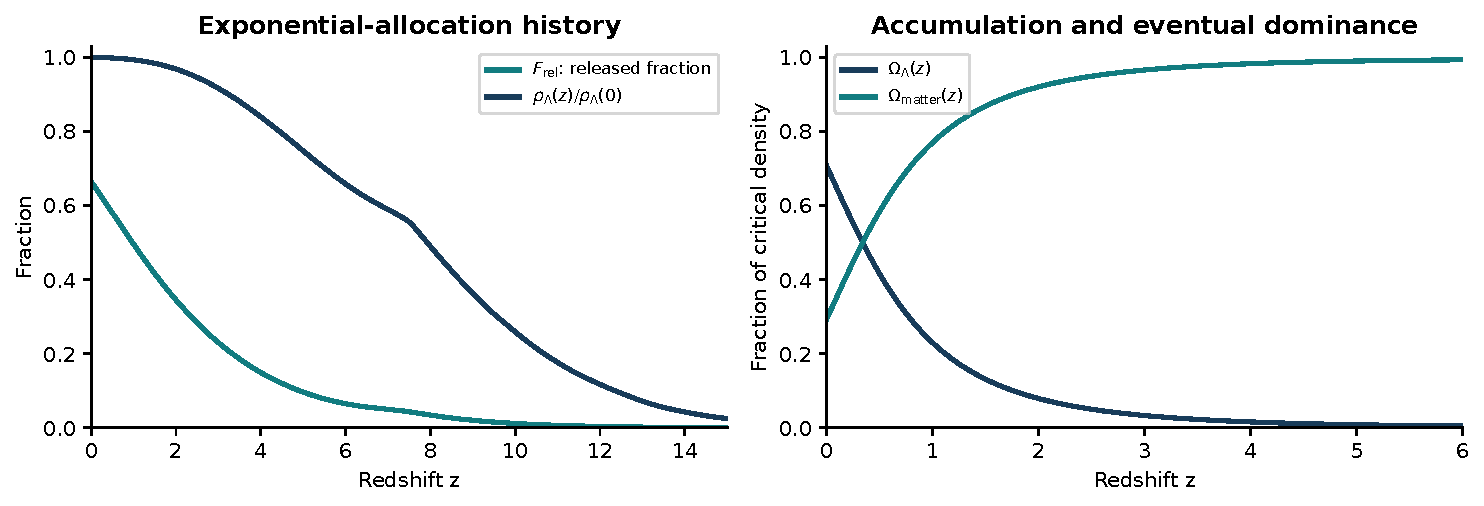
\includegraphics[width=\textwidth]{figures/release_history.pdf}
\caption{The fitted exponential-allocation release history from the
table. The released fraction counts cohorts; the vacuum density weights
their release by the physical matter density at that epoch. The right
panel shows why a substantial early vacuum density becomes dynamically
important only much later. These curves condition on the fitted kernel
and fixed reference assembly history.}
\end{figure}

\subsection{What the hydrodynamic measurement finds}

The archived Gadget-4 calculation measures progenitor information during
self-gravitating assembly. It follows $2\times96^3$ particles in a
$0.75\,h^{-1}$ comoving Mpc box, from initial conditions at $z=63$ to
$z=6$, with 48 analysis snapshots between $z=15$ and 6. Primordial
hydrogen/helium cooling and a star-formation prescription are included.
The cohort consists of the gas particles in a host at first entry.
Progenitor labels come from group membership one dynamical time earlier;
ungrouped gas is divided into spatial octants. Several partitions of
the current host measure the remaining label information. \source{C2}

Approximately half of the resolved label information is already lost at
entry. The measured kernels are fitted by
\begin{equation}
K_{\rm mix}(\tau)=1-(1-K_0)e^{-\tau/\tau_{\rm mix}},
\qquad K_0\simeq0.5.
\end{equation}
The subsequent decay takes a few dynamical times. Because this kernel
includes an immediate component, its fitted tail time cannot be directly
equated with the pure-exponential $f$ in the cosmological fit. The
appropriate comparison convolves each measured kernel with its
corresponding first-entry history.

\begin{table}[htbp]
\centering\small
\begin{tabular}{lrrr}
\toprule
Retention gate & Hosts & $I_{\rm rel}$ across partitions & Reference target \\
\midrule
$17\,\kms$ & 3 & $75.4$--$75.9$ & $94.2$ \\
$14\,\kms$ & 10 & $93.1$--$96.7$ & $94.2$ \\
$12\,\kms$ & 16 & $108.0$--$109.9$ & $94.2$ \\
\bottomrule
\end{tabular}
\caption{The measured mixing histories after convolution with assembly.
Ranges show changes among spatial partitions, not statistical confidence
intervals. Retention gates were imposed in the analysis.}
\end{table}

At the reference $17\,\kms$ gate, the measured integral is about $20\%$
too small. A $14\,\kms$ gate brings it into the required range. That
agreement identifies a physical possibility, but selecting a gate after
examining the integral does not independently predict its normalization.
At the reference gate, changing the lookback time of the labels moves
the integral to $82$--$83$; using only grouped gas moves it to $57$--$65$.
The definition of the retained source record is therefore consequential.

The run resolves only about 500--2400 gas particles per host, includes
three hosts at the reference gate, and omits molecular cooling, feedback,
and explicit subgrid diffusion. Its spatial partitions scale with the
evolving halo radius. A physical prediction requires label and resolution
rules fixed by the theory, gas-retention thresholds measured from the
simulation, and convergence under improved gas resolution and transport
physics. The present run supports a measurable assembly-and-mixing
mechanism while leaving its absolute release rate unsettled.

\begin{figure}[htbp]
\centering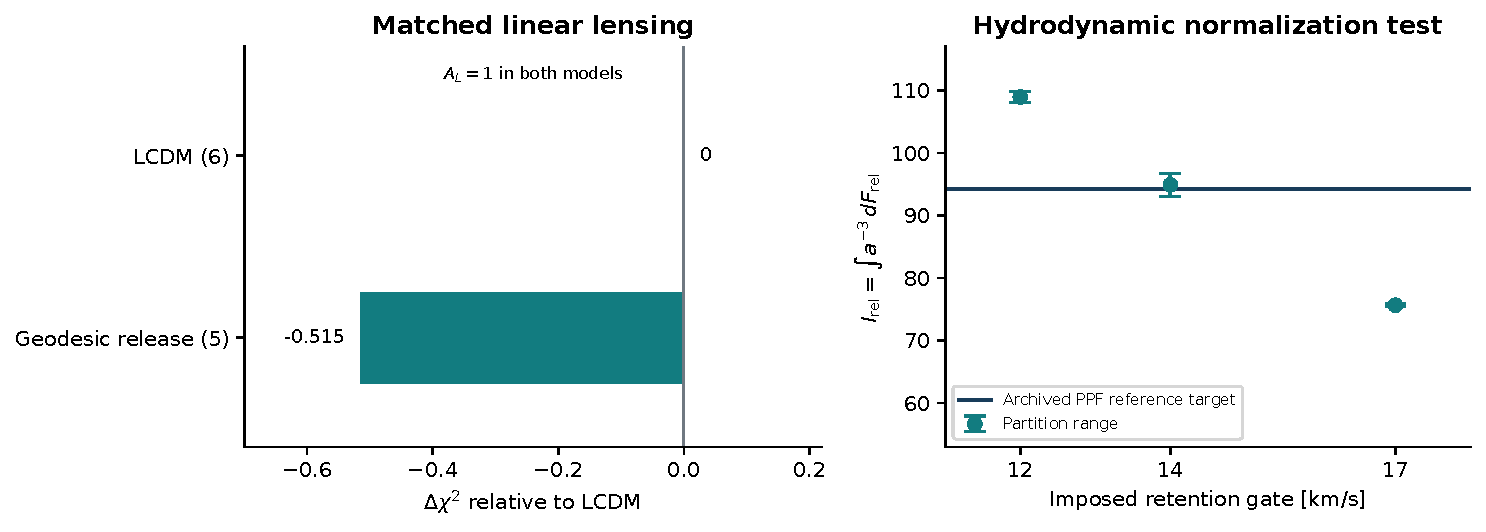
\includegraphics[width=\textwidth]{figures/cosmology.pdf}
\caption{Left: the matched linear-lensing likelihood comparison, with
cosmological parameter counts in parentheses. Right: the archived
hydrodynamic kernels compared with the linear-depletion PPF reference
target $I_{\rm rel}=94.2$. The ranges describe partition choices; the
positive-allocation model uses a different weighted integral.}
\end{figure}

\subsection{The vacuum density from the retention gate}
\label{sec:coolinggate}

Equation~\eqref{eq:flatness} turns the release integral into a vacuum
density. With $\omega_b=0.02238$ and the tied abundance, $I_{\rm rel}$
alone fixes $h$ and $\Omega_\Lambda$. The integral weights each released
cohort by the matter density at its release, $a^{-3}$, so the earliest
retaining halos dominate it. Their number is set by the retention gate,
the threshold above which a halo keeps cooling gas in which progenitor
labels mix. A lower gate admits more halos at earlier times and raises the
integral.

The construction places records in condensed baryons: stars and gas that
has cooled. Shock-heated gas whose cooling time exceeds its dynamical time
carries none. A newly assembled halo therefore enters the release history
when its virialized gas can cool within one dynamical time. This is the
atomic-cooling limit of first-galaxy formation. For primordial gas in
collisional ionization equilibrium, with atomic hydrogen and helium
cooling \cite{katz96}, Compton cooling on the microwave background, and
no molecular hydrogen or ultraviolet background, the condition
$t_{\rm cool}=R_{\rm vir}/V_{\rm vir}$ at the mean virial gas density gives
$T_{\rm gate}=(0.99$--$1.07)\times10^4\,$K for $30\ge z\ge8$. Collisional
excitation of hydrogen sets this temperature. Its rate rises by three
orders of magnitude between $8\times10^3$ and $1.5\times10^4\,$K, so the
threshold barely moves with density or redshift. The virial relation
$T_{\rm vir}=\mu m_pV_{\rm vir}^2/2k_B$ converts it to a circular velocity.
Gas at the threshold is nearly neutral, $\mu=1.22$, which gives
$V_{\rm gate}=11.6$--$12.0\,\kms$. The reference gate of $17\,\kms$ is the
same temperature evaluated for fully ionized gas, $\mu=0.59$.

The archived run measures a condensation threshold. Its group catalogues record
the star-forming gas and stellar mass of every group at each snapshot.
The fraction of groups holding condensed baryons rises from below $0.1$
to unity across $0.03\,$dex in virial velocity and reaches one half at
$8.6$, $8.9$, $9.3$ and $10.2\,\kms$ for $z=11$--15, 9--11, 7.5--9 and
6--7.5. Halo centres are denser than the virial mean, so gas condenses
in smaller halos than the mean-density estimate allows. Using this
threshold as the release gate assumes that condensed baryons identify
recoverable source records.

Table~\ref{tab:coolinggate} recomputes the first-entry history at each
pre-reionization gate and convolves it with the measured kernels. The
post-reionization gate stays at $30\,\kms$ and reionization at
$z_{\rm re}=7.66$. The six kernels measured on the ten hosts at $14\,\kms$
and the sixteen hosts at $12\,\kms$ change $I_{\rm rel}$ by at most $6\%$
at fixed gate, so the gate controls the result. The three hosts at
$17\,\kms$ have a slower tail and give the integral $75.4$--$75.9$ listed
above.

\begin{table}[htbp]
\centering\small
\begin{tabular}{lrrrr}
\toprule
Origin of the pre-reionization gate & $V_{\rm gate}$ ($\kms$) & $I_{\rm rel}$ & $h$ & $\Omega_\Lambda$ \\
\midrule
Run, condensed baryons, $z=9$--15 & 9 & $128.6$--$135.7$ & $0.77$--$0.79$ & $0.766$--$0.775$ \\
Run, condensed baryons, $z=6$--9 & 10 & $118.9$--$125.4$ & $0.75$--$0.77$ & $0.752$--$0.761$ \\
Cooling criterion, neutral gas & 12 & $103.7$--$109.5$ & $0.71$--$0.73$ & $0.725$--$0.736$ \\
Gate selected by the likelihood & 14 & $92.4$--$97.5$ & $0.69$--$0.70$ & $0.702$--$0.713$ \\
Ionized conversion of cooling temperature & 17 & $80.9$--$85.3$ & $0.65$--$0.67$ & $0.673$--$0.685$ \\
\bottomrule
\end{tabular}
\caption{Release integral, Hubble parameter and vacuum fraction from
Equation~\eqref{eq:flatness} against the pre-reionization retention gate.
Ranges span the six kernels measured at the $12$ and $14\,\kms$ gates.
The archived linear-depletion likelihood requires $I_{\rm rel}=94.2\pm0.8$, $h=0.689$ and
$\Omega_\Lambda=0.707$.}
\label{tab:coolinggate}
\end{table}

Both gates computed without feedback lie below the gate that the
likelihood selects. The cooling criterion gives $\Omega_\Lambda=0.73$ and
the run gives $0.75$--$0.77$. Supernova feedback and photoheating inside
ionized regions before the global reionization redshift remove gas from
the smallest halos and raise the effective gate
\cite{thoul96,okamoto08}. The run contains neither process. Gates from
$12$ to $17\,\kms$ span the neutral and ionized conversions of the
cooling temperature. Across that range $\Omega_\Lambda=0.67$--$0.74$, and
the vacuum density lies between $14\%$ below and $16\%$ above the
likelihood value.

The cooling-criterion calculation uses $\eta_*$, the formation abundance,
assembly of the measured fluctuation spectrum, the measured mixing kernel
and the atomic-hydrogen cooling threshold. It gives
$I_{\rm rel}=103.7$--$109.5$, $10$--$16\%$ above the archived target
$94.2$, and $\Omega_\Lambda=0.725$--$0.736$ against $0.707$. Condensation
in the no-feedback run gives $I_{\rm rel}=118.9$--$135.7$. Neither
calculation includes feedback. The likelihood selects a gate of
$14\,\kms$, about $5\times10^7\Msun$ at $z\simeq10$.

A retained well is a halo that keeps gas able to cool, in which
progenitor labels mix. The post-reionization gate measures this retention
for photoheated gas \cite{okamoto08}, and the same criterion holds before
reionization. Stars carry records and are collisionless, so they supply
no label mixing; a halo that forms a few stars and then loses its gas
lies outside the gate. The fraction of halos holding star-forming gas
therefore measures the pre-reionization gate. The Renaissance simulations
follow Population~III and metal-enriched star formation with radiative
transfer, radiative and supernova feedback, metal cooling and
Lyman--Werner backgrounds to $z=15$, $12.5$ and $8$ in rare-peak, normal
and void regions \cite{oshea15,xu16}. About $10\%$ of halos of
$10^7\Msun$ host star formation younger than $20\,$Myr, about half of
those of $10^8\Msun$ do, and all above $10^{8.5}\Msun$ do, nearly
independently of redshift and region. Treating this occupation as the
probability that a trajectory's gate lies below a given mass, and using
the linearity of the release integral in the first-entry history,
Table~\ref{tab:retentiongate} gives the result. No input in the chain is
adjusted to the vacuum density.

\begin{table}[htbp]
\centering\small
\begin{tabular}{lrrr}
\toprule
Pre-reionization gate & $I_{\rm rel}$ & $h$ & $\Omega_\Lambda$ \\
\midrule
Sharp, $10^{7}\Msun$ & $137$--$145$ & $0.81$ & $0.78$ \\
Sharp, $10^{7.5}\Msun$ & $104$--$109$ & $0.72$ & $0.73$ \\
Sharp, $10^{8}\Msun$ & $80$--$84$ & $0.66$ & $0.68$ \\
Renaissance occupation & $92.3$--$97.4$ & $0.693$ & $0.709$ \\
\bottomrule
\end{tabular}
\caption{Release integral, Hubble parameter and vacuum fraction with a
mass gate before reionization. The post-reionization gate is
$30\,\kms$ and $z_{\rm re}=7.66$. Ranges span the six measured kernels.
The likelihood requires $I_{\rm rel}=94.2\pm0.8$, $h=0.689$ and
$\Omega_\Lambda=0.707$.}
\label{tab:retentiongate}
\end{table}

The kernels move the occupation result by $\pm2.5$ in $I_{\rm rel}$, the
shape of the occupation curve by $+4/-2.4$, the reionization redshift
$z_{\rm re}=6.94$--$8.40$ by $\pm5.5$, and a post-reionization gate of
$25$--$35\,\kms$ by $\pm4.3$. In quadrature,
\begin{equation}
I_{\rm rel}=95.5\pm8,\qquad \Omega_\Lambda=0.709^{+0.017}_{-0.019},
\qquad h=0.693\pm0.021,
\end{equation}
against the required $94.2$, $0.707$ and $0.689$. Every term of the
flatness sum is fixed once the baryon density is measured: the tie gives
the committed density $5.333\,\omega_b$, the release gives
$\omega_\Lambda=\eta_*\omega_cI_{\rm rel}$, and flatness gives $h^2$ as their
sum. The boxed $h$ is therefore a prediction,
$H_0=69.3\pm2.1\,\mathrm{km\,s^{-1}\,Mpc^{-1}}$, with no fitted dark-sector
parameter, and $h$ varies nearly as $\omega_b^{1/2}$. The reionization
redshift and the post-reionization gate dominate the error. The Milky Way
satellite census places the half-occupation peak mass for any star
formation near $10^{7.5}\Msun$ \cite{nadler20}; those faint galaxies form
a few thousand solar masses of stars and lose their gas, so they lie
below the retention gate. For comparison, the standard quantum estimate
of the vacuum energy exceeds the measured value by about $10^{120}$, and
\LCDM\ fits $\Omega_\Lambda$ as a free constant. A measured cold-gas
retention fraction at $z\ge8$, a tighter reionization redshift and a
feedback-resolved mixing kernel sharpen the test; a converged integral
that differs from the target by more than its uncertainty falsifies the
normalization.

The occupation gate, the measured kernels and the post-reionization gate
fix the release history once the reionization redshift is given, and the
optical depth measures that redshift. Taking $z_{\rm re}$ from the fitted
$\tau$ removes the mixing time, and the release model has four
cosmological parameters against six for \LCDM. In the matched likelihood
with $\sum m_\nu=0.06\,$eV, nonlinear lensing and free calibration the
frozen history gives $\chi^2=2240.100$ against $2239.031$ for \LCDM,
$\Delta\chi^2=+1.07$, at $z_{\rm re}=8.12$, $\tau=0.0587$, $I_{\rm rel}=92.0$
and $H_0=68.42$. With massless neutrinos, fixed calibration and the
low-redshift offset it gives $2226.483$ against $2226.767$. The extreme
kernels and post-reionization gates of $25$--$35\,\kms$ give
$\Delta\chi^2=+1.1$ to $+2.6$. Holding $z_{\rm re}$ at $7.66$ independently
of $\tau$ gives $\Delta\chi^2=+20.2$ and $+4.0$, so the frozen history
predicts that a larger optical depth accompanies a smaller vacuum density.
With $a_0=\epsilon cH_0$ the first fit gives
$a_0=1.249\times10^{-10}\,\mathrm{m\,s^{-2}}$, and the astrophysical chain
without cosmological data gives $(1.27\pm0.04)\times10^{-10}\,\mathrm{m\,s^{-2}}$,
against $1.20\times10^{-10}\,\mathrm{m\,s^{-2}}$ from rotation curves
\cite{lelli17}. Neither uses galactic data.
\source{C2, C7, C8}

\subsection{Equation of state, vacuum energy, and decisive tests}

The vacuum stress has intrinsic $w_\Lambda=p_\Lambda/\rho_\Lambda=-1$.
Its density grows because it receives energy. If one describes this
growing density by a fictitious separately conserved fluid, its inferred
equation of state is
\begin{equation}
w_{\rm eff}=-1-\frac{1}{3}\frac{d\ln\rho_\Lambda}{d\ln a}
=-1-\frac{Q}{3H\rho_\Lambda}\le-1.
\end{equation}
This effective phantom sign comes from energy transfer. A reconstructed
decrease of the physical vacuum density would contradict the monotone
release law, provided the matter transfer and observational systematics
were modeled consistently. A fitted $w_0,w_a$ curve under conserved-CDM
assumptions is a different inference problem; its crossing of $-1$
cannot alone decide this interacting model.

Normalized microscopic probabilities are unchanged by a common shift
of their energy origin. Coupling to gravity also requires the absolute
stress-energy assigned to that origin. The current cosmological
construction selects zero initial vacuum density and generates the
subsequent density through release. Establishing that selection from the
microscopic gravitational theory remains necessary to claim a solution
of the absolute vacuum-energy problem. The empirical fit tests the
generated component under the selected initial condition.

The saved exponential-allocation calculation evolves the geodesic-clock perturbations with
zero rest-frame sound speed and $A_L=1$. Nonlinear lensing corrections
are disabled in both models, and the late-radiation truncation that
introduced reference-split dependence is disabled. The assembly table
retains its reference power spectrum while cosmological parameters vary.
Both models use massless neutrinos with $N_{\rm eff}=3.044$ and the
same simplified low-$\ell$ treatment. \source{C4, C5}

A full test requires a validated nonlinear response, assembly recomputed
for the sampled cosmology, the full low-$\ell$ likelihood, and an
independently measured release kernel. The selected depletion completion below inherits the cold linear fit;
its nonlinear spatial predictions require a separate test.
The present result demonstrates near-equal fit quality with a
microscopically tied abundance and a physically interpretable release
parameter in the specified pipeline.

\subsection{A self-limiting local completion and its coupling}
The unit-clock action is exact above a selected depletion threshold.
For $X=-\nabla_\mu\phi\nabla^\mu\phi/2$, a covariant continuation is
\begin{equation}
P=\lambda X-e-V,\quad L=3(K-V)>0,\quad
e=\frac\lambda2+\frac{2[L-\lambda]_+^3}{3L^2},\quad \lambda\ge L/2.
\end{equation}
The constant $K$ is a minimum total energy. For $\lambda>L$ the
Lagrangian is exactly $\lambda(X-1/2)-V$. On the intermediate branch
$r=\lambda/L\in(1/2,1)$, define $v=\sqrt{2X}$ and $j=\lambda v$.
Then $X=1/2-2(1-r)^2$ and
\begin{equation}
\dot j=-\left[\theta+\frac{V_\phi A(r)j}{\lambda^2}\right]j,
\qquad A(r)=\frac{1+2r-2r^2}{3-2r}\in[3/4,1].
\end{equation}
For regular flow with $K-V$ bounded away from zero, the current stays
nonnegative. Its depleted homogeneous endpoint has $j=0$,
$\rho=K$, $p=-K$. The regular sound speed lies between zero and one.
The constant minimum removes the scalar force at rest. This slows the
source field relative to proper time; no universal atomic-clock effect
has been established. The cubic and floor are constitutive choices.
\source{D1}

For the fitted history, the choice
$K=V(1)+B[e^{-\eta_*F(1)}-e^{-\eta_*}]$ bounds all remaining future
release under the stated monotonicity assumptions. The saved value is
$K=0.3369964$ in units $3H_{100}^2/(8\pi G)$, with
$\max_{a\le1}L/\bar C=0.0299937$. The background and a neighborhood of
its linear perturbations stay on the original branch. Hence the
completion inherits the fitted cold adiabatic linear cosmology. Deep
voids enter a pressure regime with a changed minimum energy and require
new expansion, profile, and lensing predictions. Nonzero-null-gradient
interfaces and nonlinear caustics remain unresolved.

A finite-work contact extends this mechanism to redistribution. For
a transition $E\to E'$ toward target $h$, let
$Q=\Theta\ln(h'/h)$, $W=E'-E+Q$, $U'=U-W$, and $E_B'=E_B+Q$.
Their total energy is conserved. A symmetric gate $v(U)v(U-W)$ allows
only admissible endpoints and vanishes at the floor. Central pair
impulses give reciprocal momentum exchange. The target and physical
rate require selection beyond detailed balance. \source{D2}

A warm fluid stress stores heat as $e_T=z n^\gamma\ge0$ with
$1<\gamma\le2$ and
$\rho=R_0(n,\phi)+e_T$, $p=p_0+(\gamma-1)e_T$.
Its sound speed is an enthalpy-weighted average of the cold speed squared
and $\gamma-1$, preserving the causal local bound and energy floor.
The gate $g=n\mu/(\lambda_0+\gamma e_T)\in[0,1]$ retains a regular
signed power $gB_c$ and reduces to the cold $v_0^2$ gate.
In the selected $\gamma=4/3$ compression test, five resolutions up to
2048 cells conserve mean total energy to $4.9\times10^{-15}$ and keep
positive current. Generated heat falls from 0.0641 to 0.0140 under
refinement, so physical dissipation has not converged. A separate
particle-feedback test has fractional energy error $1.02\times10^{-5}$
and stops short of the target when available work is insufficient.
These tests establish a conservative effective implementation; the
coupled spatial and multistream evolution remains to be validated.
\source{D2}

\section{Clusters: conservative dynamics and observed targets}
\label{sec:clusters}

The cluster calculation uses positive, inertial stock, gas, and stars in
one gravitational potential. Gas pressure and shocks can separate the
gas from the weakly coupled stock and galaxies during an encounter.
The observed lensing map measures their total projected mass. This
construction supplies a transport mechanism and quantitative targets;
the present comparisons do not constitute a fitted cluster population.
\source{CL1--CL3}

\subsection{A common mass budget and a conservative encounter}
For a fully released closed cohort, the adopted normalization in the
formation mass convention of the cosmological fit is
\begin{equation}
k_C=5.333\,e^{-\eta_*}=5.1760752,\qquad C_0=k_C B_0.
\end{equation}
The bare convention gives $e^{-\eta_*}/\epsilon=5.164$.
If its baryons and stock remain coextensive, the baryon fraction is
$1/(1+k_C)=0.1619151$. More generally, an aperture retains different
fractions of the ancestral components. The measured target can be
expressed as
\begin{equation}
C_{\rm req}=M_{\rm grav}-B,\qquad
\eta_{\rm ret}=\frac{k_C B}{C_{\rm req}}
=\frac{f_b^{\rm ret}}{f_C^{\rm ret}}.
\end{equation}
This distinguishes the common cohort normalization from the distribution
produced by assembly. A positive inventory exists for $C_{\rm req}>0$:
$B_0=\max(B,C_{\rm req}/k_C)$ leaves nonnegative exterior baryons
$B_0-B$ and stock $k_CB_0-C_{\rm req}$. It does not determine a
realizable transport history or its energy cost.

The encounter model uses central pair impulses with opposite momentum
changes. If $w$ is the radial relative velocity and $\mu$ the reduced
mass, the kinetic change is $\Delta K=\mu(w'^2-w^2)/2$. Explicit work
and heat registers balance that change, and a symmetric gate suppresses
transitions with an endpoint at the energy floor. Gas and stars from
either progenitor can be local partners. The target distribution, rate,
range, and initial work reserves are selected effective inputs.
\source{D2, CL1}

Fourteen encounters and three isolated controls test a common Plummer
mass ratio of 0.3, with 1344 particles at baseline and 2688 in the
resolution control. Weak contact leaves stock near the galaxies while
gas lags. A floor-state run permits no events and reproduces the
no-contact evolution; a low-work run permits 61 events against 7114
with the larger reserve. The largest energy drift is below 0.007\%
of the binding energy; pair momentum conservation holds at roundoff.
The strongest tested contact changes the isolated stock median radius
by $-27\%$ and gas median radius by $+46\%$ in six dynamical time units.
That control prevents interpreting a higher contact rate as an established
cluster solution. The particle encounters test the finite-work coupling;
they do not evolve the full spatial stress of the depleted scalar.

\subsection{X-COP profiles and independent weak-lensing masses}
The public X-COP archive supplies twelve hydrostatic radial profiles,
seven with stellar mass data. Five overlap the MENeaCS lensing catalogue.
The comparison adopts the observational distance convention
$H_0=70\,\kms\,\mathrm{Mpc}^{-1}$ and $\Omega_m=0.3$.
Projected stellar masses are approximately deprojected using the stated
profile model. Unmeasured intracluster light, hydrostatic departures,
triaxiality, and profile covariance remain relevant.
\cite{xcopnew,herbonnetnew}\source{CL2}

All nominal NFW hydrostatic targets admit positive cumulative stock and
positive stock in fifteen tested shells. At the hydrostatic $R_{500}$,
the coextensive-to-hydrostatic total-mass ratios for A1795, A2029, A2142,
A2319, A644, A85, and ZW1215 are respectively
$0.903$, $0.912$, $1.023$, $1.213$, $0.851$, $0.952$, and $0.679$.
These reconstructed totals are inputs to a target audit, rather than
stock profiles predicted from the observed baryons.

\begin{table}[H]
\centering\small
\begin{tabular}{lrrr}
\toprule
Cluster & Coextensive $M_{500}$ & Lensing $M_{500}$ & $\eta_{\rm ret}$\\
\midrule
A1795 & 3.96--4.23 & $9.3\pm2.2$ & 0.518\\
A2029 & 7.46--8.07 & $12.1\pm2.5$ & 0.704\\
A2142 & 9.29--10.02 & $9.7\pm2.3$ & 0.969\\
A85 & 5.20--5.43 & $5.7\pm2.2$ & 0.937\\
ZW1215 & 4.19--4.46 & $3.5\pm2.2$ & 1.143\\
\bottomrule
\end{tabular}
\caption{Masses in $10^{14}\Msun$. The coextensive prescription solves
its own overdensity radius; its range doubles the nominal stellar mass
and is a sensitivity interval. Retention ratios use the nominal baryons
within each central lensing target's radius. Lensing errors are the
published NFW marginal errors. No combined exclusion significance is
assigned.}
\end{table}

\begin{figure}[H]
\centering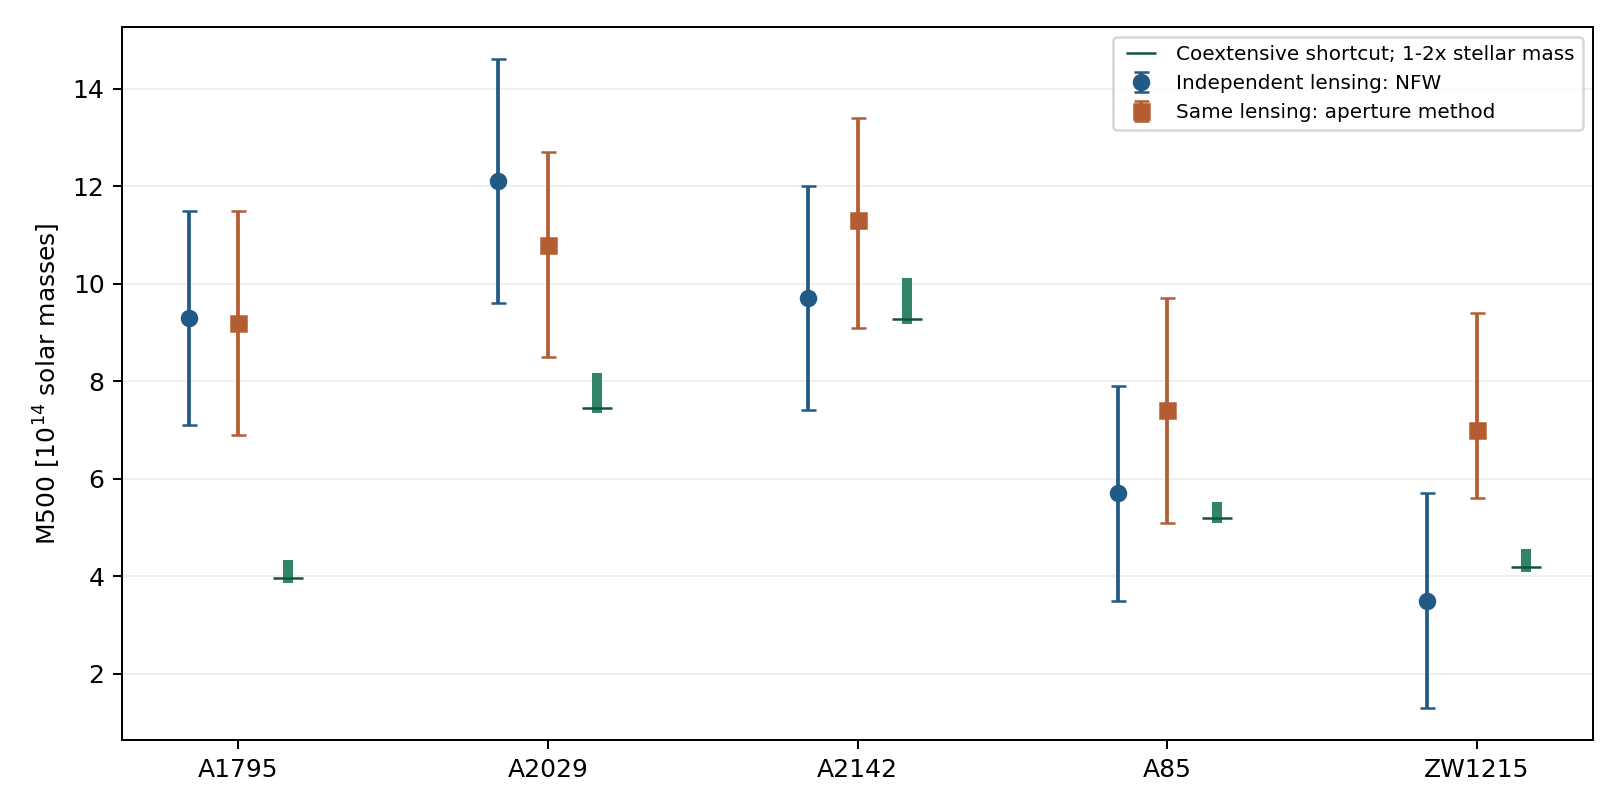
\includegraphics[width=\textwidth]{figures/cluster_lensing.png}
\caption{The common coextensive prescription and two mass estimators
from the same lensing data. Their errors are correlated. A1795 and
A2029 require a transport or reconstruction explanation; A2142 and A85
are useful normalization controls. ZW1215 is sensitive to the estimator.}
\end{figure}

\subsection{Why clusters remain fair samples}
The stock that reaches the galactic response law in isolated galaxies
(Section~\ref{sec:stockselection}) is the same stock that fills clusters.
The selection acts through the cells of active carriers, on the stock each
carrier carries. A carrier's records are identified with its condensed
baryons, stars and cold gas; virialized hot gas relaxes toward the Gibbs state
of its potential. A carrier's support ends where its records stop dominating
the enclosed baryons, and its cells act on the stock bound to the potential of
its records and the stock it carries.
In the X-COP clusters the supports and cell energies are:
\begin{center}
\small
\begin{tabular}{lcccc}
\toprule
Cluster & $r_d$ (kpc) & $r_d/R_{500}$ & condensed fraction at $R_{500}$ & cell energy ((km/s)$^2$)\\
\midrule
A85 & 47 & 0.038 & 0.025 & 21\\
A1795 & 65 & 0.056 & 0.044 & 90\\
A2029 & 76 & 0.054 & 0.052 & 93\\
A2142 & 68 & 0.048 & 0.047 & 37\\
A2319 & 99 & 0.072 & 0.035 & 121\\
A644 & 87 & 0.069 & 0.051 & 132\\
ZW1215 & 97 & 0.071 & 0.038 & 55\\
\bottomrule
\end{tabular}
\end{center}
Here $r_d$ is the radius where projected stellar mass equals gas mass, an upper
bound, and the cell energy is per unit cluster stock. Outside $r_d$, and for
stock crossing it unbound, the cluster stock is collisionless and keeps the
cohort ratio of the common mass budget. The X-COP medians test that ratio:
\begin{center}
\begin{tabular}{lcc}
\toprule
& total/baryon & source\\
\midrule
Cohort prediction $1+k_C$ & 6.18 & theory\\
X-COP median, $R_{500}$ & 6.45 & hydrostatic, $f_\star=0.015$\\
X-COP median, $R_{200}$ & 6.10 & hydrostatic, $f_\star=0.015$\\
Response law at $R_{500}$ ($g_{\rm bar}=0.05$--$0.07\,a_0$) & 4.2--5.0 & theory\\
Cohort stock plus an always-on response & 9.4--10.2 & theory\\
\bottomrule
\end{tabular}
\end{center}
A response acting on cluster stock fails in either direction. Galaxy
outskirts that obey the law lie at the same $g_{\rm bar}/a_0$, at 35--50\,kpc in
a Milky Way model, so the switch cannot depend on acceleration alone.

Contact runs start from the observed profiles of the seven clusters with the
archived contact kernel, conservative softened gravity and fixed baryons, and
compare with matched no-contact controls after 8--10\,Gyr, at three contact
proposals per orbit:
\begin{center}
\small
\begin{tabular}{lccc}
\toprule
Rule & $R_{500}$ & $0.3R_{500}$ & $0.1R_{500}$\\
\midrule
Cells throughout, galactic work allowance & 0.547--0.787 & 0.319--0.440 & 0.209--0.366\\
Support only, galactic work allowance & 0.976--0.997 & 0.867--0.961 & 0.369--0.731\\
Support only, cell work & 0.997--1.007 & 0.990--1.019 & 0.563--0.937\\
Support, carried stock, cell work & 0.9998--1.0008 & 0.997--1.002 & 0.985--1.007\\
\bottomrule
\end{tabular}
\end{center}
\begin{figure}[H]
\centering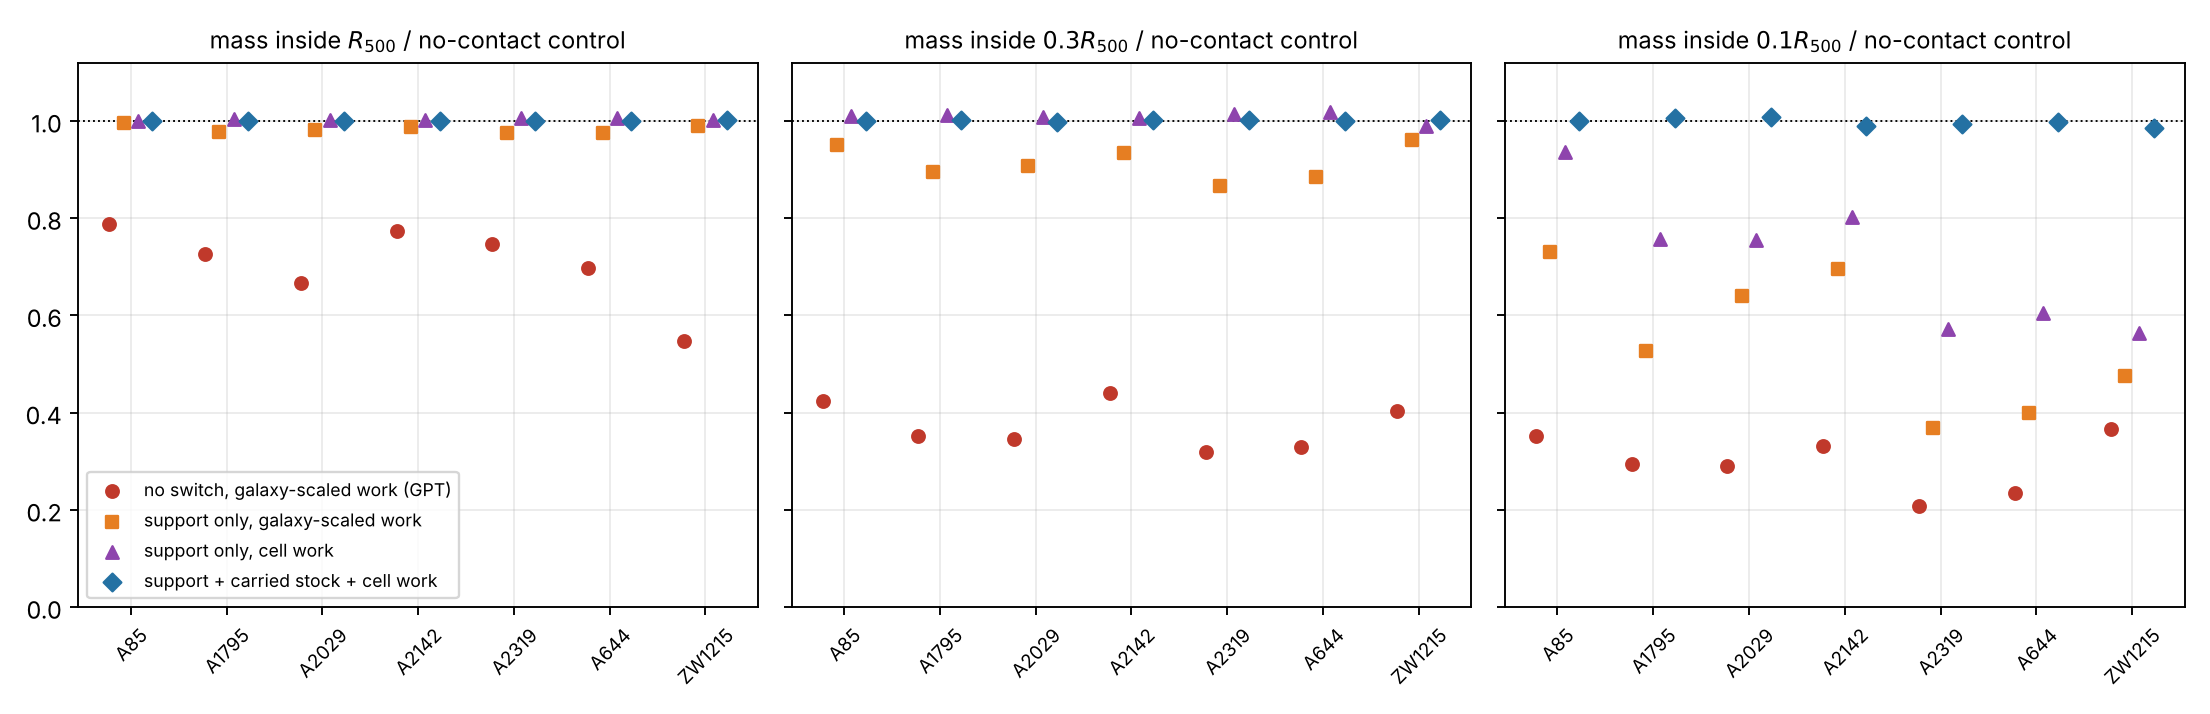
\includegraphics[width=\textwidth]{figures/cluster_switch.png}
\caption{Mass inside three radii relative to the no-contact control for the
four rules of the table, with 2000, 2000, $10^4$ and $1.6\times10^4$
particles.}
\end{figure}
Contacts are confined to 4--7\% of $R_{500}$ with $10^{-4}$ of the binding
energy, so the outer result follows from the support. With support only, the
central galaxy's cells drain the uncarried cluster stock in its support to
7--30\% of the control. With carried stock, averaged over 8--10\,Gyr, the core
keeps 94--105\% inside $r_d$ and 99--101\% inside $2r_d$, with a Poisson error
of 6--14\%. The central galaxy's carried stock falls from 1.1--4.3 to
0.57--0.85 times its galactic-law value, and its support keeps 7--11 times
that value in uncarried stock. The same rule leaves isolated galaxies on the
law inside their supports, which for the Milky Way end at 115--490\,kpc.
The X-ray ellipticals on the radial acceleration relation \cite{lelli17}
test the record identification directly. Over the radii used there, stars
dominate their enclosed baryons; in NGC~720 hot gas becomes the dominant
baryonic component only outside about 200\,kpc \cite{humphrey11}. Excluding
the hot gas from the record source lowers the outermost points by at most
0.04\,dex. Isolated ellipticals hold no group stock and should follow the law
out to the radius where their hot gas dominates. Carrier support
makes four observational distinctions:
\begin{itemize}
\item central galaxies of groups and brightest cluster galaxies depart
from the rotating-galaxy relation, with an acceleration scale about
17 times larger for brightest cluster galaxies \cite{bcgrar,centralsrar};
\item X-ray groups at 0.5--2\,keV require mass beyond the response law
\cite{angus08}, as retained collisionless stock supplies;
\item in X-ray groups the excess over the law begins in the core: in A262,
MKW4 and RXJ1159.8+5531 it exceeds 0.1\,dex within 5--13\,kpc, while hot gas
overtakes the condensed baryons only at 85--210\,kpc
\cite{gastaldello07,vikhlinin06}, so the excess traces the uncarried group
stock;
\item isolated ellipticals follow the law out to the radius where their hot
gas outweighs their stars; NGC~720 lies within about 0.1\,dex of it at
102\,kpc in mass models extrapolated beyond the X-ray data \cite{humphrey11}.
\end{itemize}
Resolved member galaxies and cosmological assembly are the open parts.
\source{G8, G9, G10, G11}

\subsection{What the outliers require}
The central A1795 and A2029 lensing targets require respectively
48.2\% and 29.6\% of the minimal cohort's initial baryons outside the
aperture; for A1795 this is $7.87\times10^{13}\Msun$. Twelve finite
transport maps preserve positive marginals for the seven hydrostatic
and five lensing targets. This inventory construction leaves the
assembly time and work requirement undetermined. \source{CL3}

The gas must obey the same total potential,
\begin{equation}
a_g=-g-\frac{P_{\rm th}'+P_{\rm nt}'}{\rho_g}+\frac{f_{Cg}}{\rho_g}.
\end{equation}
Segregation, acceleration, and reciprocal contact are possible contributions.
Passive drag vanishes at zero drift, so stationary contact support requires
its own physical law. XRISM's low turbulent support in A1795 and A2029
constrains a purely turbulent explanation. \cite{sarkarnew,xrismnew}
The conditional pressure audit also depends on inner lensing extrapolation
and thermal reconstruction; a joint fit remains open.

A644's 58-knot forward profile contains 11 negative total-mass increments
and 15 negative stock increments. A monotone reconstruction requires
2.156 marginal error units of maximum displacement; absent joint
covariance, this is not an exclusion significance. Positive parametric
profiles require comparison with the underlying gas data. For ZW1215,
at 1320 kpc the correlated NFW-lensing, aperture-lensing, and hydrostatic
estimates are $4.32$, $7.0$, and $7.41\times10^{14}\Msun$. Both systems
retain reconstruction uncertainty rather than a new gravity coefficient.

\subsection{The Bullet Cluster supplies a spatial target}
The CANUCS Bullet v1 best-fit maps separate a total lens reconstruction
from a supplied gas component. At lens redshift 0.296 and
$D_{ls}/D_s=1$, their normalization gives
$\Sigma_{\rm crit}=1.8268761\times10^9\Msun\,\mathrm{kpc}^{-2}$
and $1''=4.41302$ kpc. Registered apertures around BCG3 give
\begin{center}
\begin{tabular}{lrrr}
\toprule
Radius & $M_{\rm total}/10^{13}\Msun$ & $M_g/10^{13}\Msun$ & Gas fraction\\
\midrule
60 kpc & 2.151 & 0.099 & 0.046\\
150 kpc & 8.511 & 0.618 & 0.073\\
\bottomrule
\end{tabular}
\end{center}
The released subcluster halo centre lies 3.92 kpc from BCG3. The
supplied gas-density map peaks about 169 kpc away within the specified
search region, with an 8.68 kpc gas pixel. This is a density-map
diagnostic, rather than an X-ray brightness peak or an offset posterior.
Subtracting gas leaves a component that still includes stars.
\cite{bulletnew}\source{CL2}

\begin{figure}[H]
\centering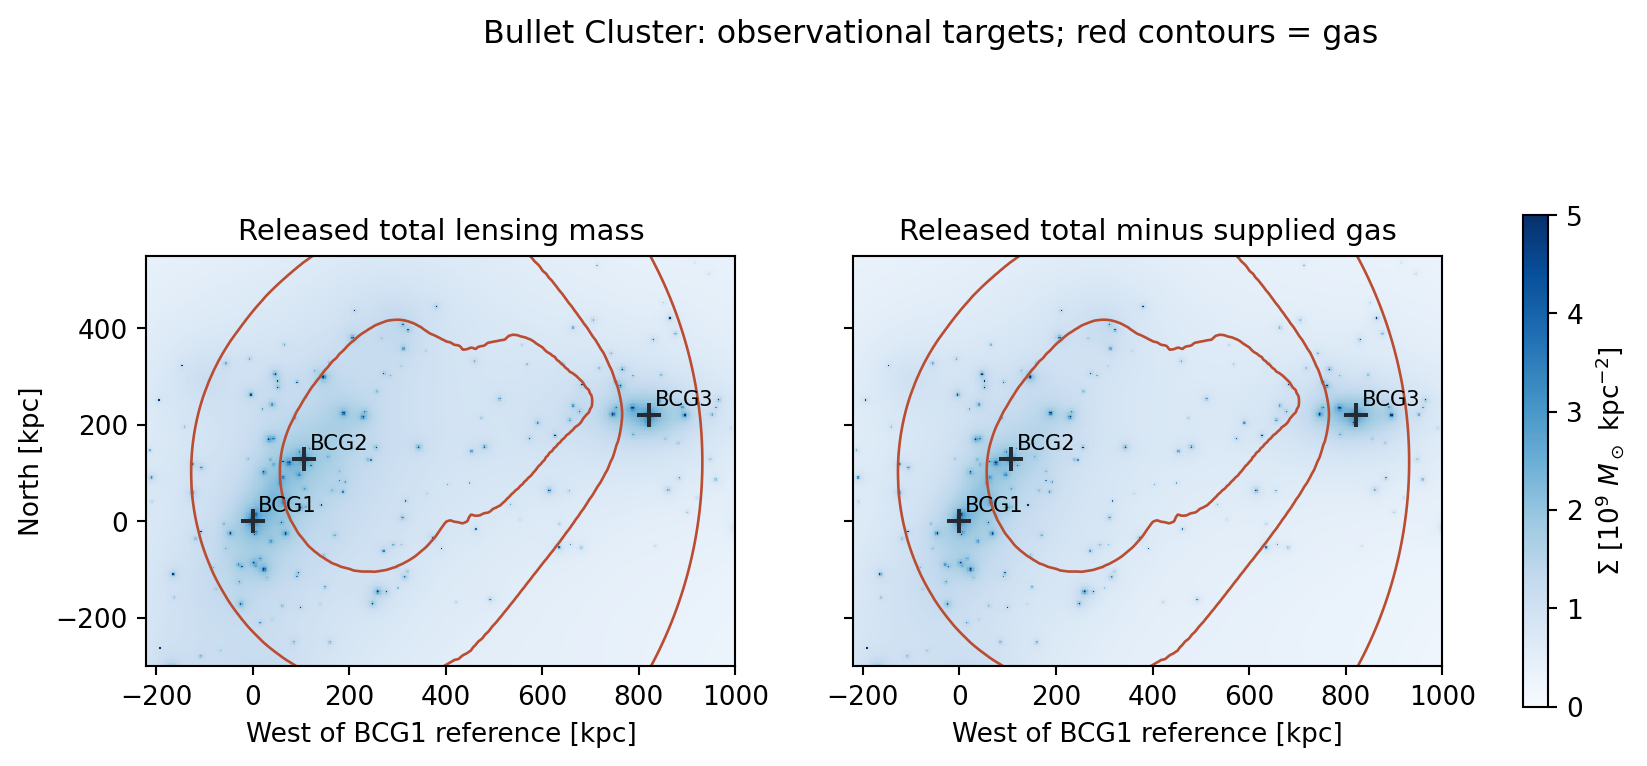
\includegraphics[width=\textwidth]{figures/cluster_bullet.png}
\caption{Observed targets from the released Bullet v1 lens model.
The red contours show its supplied gas component. Both panels are
derived from the public reconstruction; no simulated map is fitted here.}
\end{figure}

Aperture masses change by at most 0.214\% under pixel coarsening; this
is a numerical check and excludes observational uncertainty. Under an
illustrative $10^{15}\Msun$, 300 kpc scaling, the encounter calculations
have 24--30 kpc force softening and roughly 90 kpc map smoothing. They
cannot establish agreement with the few-kiloparsec halo--galaxy alignment.
A successful forward test must preserve isolated cluster profiles and
then reproduce lensing, gas morphology, and offsets using one selected
contact law and independently specified assembly conditions.


\section{Joint interpretation}

The empirical contribution is a common prescription that connects a
galactic acceleration scale, a retained mass distribution, tidal evolution,
and cosmological energy transfer. The calculations use the same
microscopic entropy and conversion fraction in several settings. Their
success would be more constraining than unrelated curve fits because
changing those coefficients would move several observables at once.

The LMC enclosed masses and NGC~628 vertical dispersions support
the retained-stock prescription against the tested external-field and
algebraic QUMOND comparisons. Crater II gives a favorable comparison
with a specified NFW population, with strong dependence on the error
budget. The reference acceleration-line projection agrees, while the
high-redshift catalogue test retains a residual trend. The matched
cosmology recovers CMB and distance data with a tied abundance; ACT
lensing and $E_G$ add compatible checks. These results establish the
scope of the particular comparisons summarized in Table~\ref{tab:fifteen}.
Antlia 2, cluster outliers, Galactic mass, and independent release
normalization remain active constraints.

\subsection{The derivation has identifiable physical commitments}

\begin{table}[htbp]
\small
\begin{tabularx}{\textwidth}{P{.24\textwidth}YY}
\toprule
Step & Result supplied & Physical commitment or outstanding test \\
\midrule
Finite face and cell ensemble
& $16=7+9$; 1680 cell states; $g=7.4198000$ and $\eta_*=0.02986684$.
& The spin, matching vertex, occupancy rule, closure invariant, and
evidence measure define the ensemble. \\
Horizon and transverse response
& $\epsilon=g/(2\pi)^2$; $a_0=\epsilon cH$; Bose response.
& The tilt-mode lever $\ell=g\,c/H$ in the horizon bath connects the
count to acceleration and fixes the mode energy. \\
Retained galactic stock
& An inertial positive mass component, inherited by carriers and
transported by collisionless evolution.
& Assembly budgets, carrier assignment, profile preparation, and
relaxation must be specified independently of the target observables. \\
Cosmological conversion
& $\eta=\eta_*$ and an initial abundance near $\epsilon^{-1}$.
& Common energy conversion, the selected pre-acoustic formation map
(whose microscopic vertex remains open), and the absolute vacuum
matching condition enter the physical identification. \\
Assembly and mixing
& A cumulative release function and a weighted vacuum integral.
& Retention gates, progenitor labels, and transport set the normalization;
the current expansion fit determines one mixing parameter. \\
Geometry and perturbations
& Reduced Newtonian equations and no-slip identity proved from the
specified action; carrier equations proved on their regular branch.
& The continuum embedding, constrained director dynamics, and the
physical matching of the effective actions remain separate requirements. \\
\bottomrule
\end{tabularx}
\caption{The logical connection between the microscopic model and the
observables. An exact finite calculation can coexist with conditional
physical identifications and an incomplete continuum derivation.}
\end{table}

This chain explains why the empirical results bear on the microstructure:
the model does not choose a separate acceleration coefficient for the LMC
and the redshift sample, or a separate release fraction for each
cosmological data combination. It also identifies which steps the data
cannot determine by themselves. A fit to an effective gravitational field
does not uniquely identify the microscopic state space that produced it.

\subsection{Which conventional assumptions are challenged}

For the LMC, the comparison challenges the applicability of an
instantaneous external-field suppression to a previously established
gravitating stock. A retained distribution continues to contribute after
the ambient field changes. The tested QUMOND prescriptions and the stock
model make different mass predictions with the same stated baryons.
Joint stream and reflex modeling can test that distinction more directly
than comparing scalar enclosed-mass summaries.

For Crater II, the issue is the central structure and stripping response
of the excess gravitating mass. The tested capacity profile loses enough
support to produce a cold, extended remnant under the adopted orbit and
initial conditions. Standard-concentration NFW halos under the tested
abundance prior perform poorly in that comparison. Low-concentration
and cored dark-matter alternatives require their own matched tests.
Assembly history already matters in conventional dark-matter dynamics;
history dependence alone cannot distinguish the two frameworks.

For the acceleration scale, the proposed change is a cosmological
normalization $a_0\propto H$. Its observed value at one epoch would cease
to be an independent constant. The published intermediate-redshift
relation is consistent with the fixed reference curve under the stated
projection. A direct galaxy-level likelihood would test both its curvature
and its scatter.

Irreversible source-identity loss generates vacuum energy. The microscopic
conversion and formation abundance tie the release history to the CMB
and distance fits. The halo occupation of feedback-resolved simulations sets the retention
gate with no input adjusted to the vacuum density and gives
$\Omega_\Lambda=0.709\pm0.02$ against the required $0.707$. Gates computed
without feedback give $0.73$ from the hydrogen cooling criterion and up to
$0.77$ from condensation in the archived run
(Section~\ref{sec:coolinggate}). The frozen history, with the reionization redshift taken from the fitted optical depth, fits the cosmological data with four parameters at $\Delta\chi^2=+1.07$ against six-parameter \LCDM. A measured cold-gas retention fraction sharpens this normalization test. The current evidence supports these mechanisms as
testable alternatives; it does not establish the elimination of all
dark-matter models, all MOND formulations, or the absolute cosmological
constant problem.

\subsection{A joint test of the same construction}
\label{sec:jointtest}

The reference galactic normalization uses
$H_0=67.4\,\mathrm{km\,s^{-1}\,Mpc^{-1}}$. The standard linear-depletion
configuration gives $H_0=68.458$ and
$a_0=1.25005\times10^{-10}\,\mathrm{m\,s^{-2}}$, about $1.6\%$ above
the reference acceleration scale; the 22 dwarf classifications are
unchanged and their $\chi^2$ moves by $0.1$. The catalogue diagnostics and
old-disk check use the exponential fit's normalization,
$H_0=68.93885586416$ and $a_0\simeq1.25883\times10^{-10}\,\mathrm{m\,s^{-2}}$,
with massless neutrinos, linear lensing and a low-redshift supernova offset.
The quoted $H_0$ values are in $\mathrm{km\,s^{-1}\,Mpc^{-1}}$.
Joint inference propagates the fitted $H(z)$ into galaxy assembly, the
acceleration relation and the relaxation of existing stock.

The same relation makes galaxy dynamics an independent measurement of the
Hubble constant, $H_0=a_0/\epsilon c$. The standard linear-depletion fit's $H_0=68.458$
requires $a_0=1.250\times10^{-10}\,\mathrm{m\,s^{-2}}$, and the
Cepheid-calibrated $73.04$ requires $1.334\times10^{-10}\,\mathrm{m\,s^{-2}}$.
Hubble-flow distances carry almost no information on $H_0$ here, because
the inferred $a_0$ scales with the assumed distance scale in nearly the
same way as the prediction. The 44 SPARC galaxies with tip-of-the-red-giant-branch,
Cepheid or supernova distances, fitted with per-galaxy mass-to-light
ratios, distances and inclinations under their priors, give
$a_0=(1.21\pm0.19)\times10^{-10}\,\mathrm{m\,s^{-2}}$, or
$H_0=66\pm11\,\kms\,\mathrm{Mpc}^{-1}$. All 153 galaxies of quality 1--2
give $1.03\pm0.11$, and the subsamples range from $0.97$ for gas-dominated
dwarfs to $1.37$ for massive galaxies with absolute distances; that drift
sets the present systematic floor. A $2\%$ determination of $a_0$ with
absolute distances separates $68.5$ from $73$ at $3\sigma$.
\source{T1, section 27.3}

The same requirement applies to the Milky Way potential. The available
moving-LMC calculations use a Galactic mass within 50 kpc about $17\%$
above the Brooks et al. inference in the stock model, and about $36\%$
above it in the NFW model. A joint Milky Way--LMC fit would alter the
satellite pericentres and the stripping histories. Those changes should
be propagated to both Crater II and Antlia 2 before assigning a combined
evidence ratio. \source{G4}\cite{brooks}

A decisive program follows from these dependencies:
\begin{enumerate}
\item Infer the Milky Way and LMC jointly using streams, halo reflex
kinematics, and a common source-conserving force model. Predict additional
stream observables from the resulting mass distributions.
\item Evolve the dwarf populations with resolved self-gravity and
prespecified progenitor priors. Apply the actual stellar selection,
velocity-gradient, and membership inference to their mock observations.
Include concentration scatter and physically motivated cores in the
dark-matter comparison.
\item Fit the intermediate-redshift galaxy data directly with the
cosmological $H(z)$ from the same model. Preserve correlations between
baryonic masses, pressure support, geometry, and acceleration.
\item Measure retention and source-label loss in converged hydrodynamic
runs with supernova feedback, photoheating and a label prescription fixed
in advance, and read the retention gate from gas retention. Use that release history
with the existing positive-allocation perturbation implementation and
a matched full cosmological likelihood.
\end{enumerate}
Each step tests an existing physical commitment of the construction.

\appendix
\section{Provenance and numerical verification}

\subsection{Scope of the verification}

The integrated Lean 4.35.0 library contains 160 modules and 2,937 audited theorem
constants, including its legacy sublibrary. The manuscript ledger records
874 statements as proved, 90 in part, 153 as physical premises, 64 as
data comparisons, and 19 as simulation outputs. Its other entries
distinguish numerical calculations, definitions, and statements awaiting
formalization. The saved audit reports only the standard Lean axioms
and no admitted proofs. The counts include mathematical helper results.
\source{T4}

For this paper, the relevant proofs cover the finite ensemble and closure
root, the restricted freedom in the marked-register identification,
positive finite allocation, and radial relaxation with preserved angular
marginals. First variation with compactly supported tests gives the
reduced two-potential and Newton equations. Decay at infinity gives
$\Phi=\Psi$. The carrier-action proof assumes a smooth interpolating
function; the adopted singular derivative at zero baryonic field limits
its direct classical application. The constrained director equation,
full cosmological perturbations, and observational likelihoods retain
their separate analytic or numerical status.

The numerical review independently evaluates the finite ensemble,
redshift projection, LMC mass profile and QUMOND flux, archived Crater II
likelihoods, and a reference release history. The current verification
record uses the unrounded acceleration coefficient and imports the
higher-accuracy matched cosmology endpoints. The associated figures
use those records. The archived release-history and hydrodynamic panels
retain their original linear-depletion calibration.

The dated research records include the exponential-allocation cosmological
optimization, finite-work and fluid tests, merger controls, observed cluster
reductions, and outlier audits. They were not rerun to typeset this paper.
Six extension modules contribute 119 explicit theorem declarations.
The integrated 4.35 build, source scan, axiom audit, and ledger citation
check pass; the six modules also pass standalone Lean/mathlib 4.19 checks.
The existing claim ledger retains its snapshot scope. \source{T5} Source inspection and saved
audits establish which calculation supports each statement. Numerical
convergence, selection effects, and physical matching are assessed with
the relevant empirical result. SHA-256 records preserve the identities
of the source and result snapshots.

\clearpage
\subsection{Local source key}

Paths below are relative to the supplied \path{Sol and Fable} workspace.
The source package includes the document, figures, numerical review, and
verification script; the original simulation archives remain in that
workspace.

\small
\begin{longtable}{P{.065\textwidth}P{.88\textwidth}}
\toprule
Key & Source and use \\
\midrule
T1 & \path{01 Current Papers/Full/Entropic Scalar EFT.tex}. Current microscopic
construction, effective galaxy dynamics, release accounting, and
covariant closure; especially sections 5--6, 15, 20, N.8, and O.3--O.15.
The numerical review records its source snapshot by hash. \\
T2 & \path{02 Research/Spacetime consolidation 2026-10-16/MICROSTRUCTURE_TO_SPACETIME.md}.
Finite geometry, interaction, matter, and clock
construction. \\
T3 & \path{01 Current Papers/Microstructure CDT/MICROSTRUCTURE_CDT.tex}.
Selected CDT realization, normalization conventions, and finite
geometry--matter--clock tests, with conventions aligned to the current
Entropic Scalar EFT manuscript. \\
T4 & \href{https://github.com/jakechinitz/Entropic-EFT-Lean/tree/cfcfa373eaf55adac6a2a0ddeb859766c985f71c}{Entropic-EFT-Lean, 29 October 2026 snapshot}.
Local library: \path{02 Research/Unified closure 2026-10-21/formalization}.
Claim ledger, theorem sources, and saved axiom/citation audits. \\
G1 & \path{04 Notes and References/Technical Notes/history_gravity_reproduction_2026-09-27.md}.
Analytic galaxy checks and reproducible provenance for the stock model. \\
G2 & \path{02 Research/LMC and satellites checks/qumond_flux.py} and
\path{02 Research/LMC and satellites checks/output.txt}.
External-field QUMOND surface-flux comparison. \\
G3 & \path{02 Research/Crater II and Antlia 2 vs LCDM/PREREGISTRATION.md},
\path{PREREGISTRATION.sha256}, and \path{analyse_grid.py} in that folder.
Core observation likelihood, priors, and hash identity. \\
G4 & \path{02 Research/Crater II and Antlia 2 vs LCDM/RESULTS_with_LMC.md},
\path{analyse_lmc.py}, and \path{lmc_results.zip} in that folder.
Current moving-LMC trajectories and evidence. \\
G5 & \path{04 Notes and References/Technical Notes/carrier_hierarchy_calcs_2026-09-26.md}.
The active-carrier inheritance calculation for tidal dwarfs. \\
G6 & \path{02 Research/Crater II and Antlia 2 vs LCDM/bf_robustness.txt} and
\path{antlia2_ji_mock/mock_approx_analysis.txt} in that folder.
Model-error sensitivity and approximate observational mocks. \\
G7 & \path{02 Research/Stock adjustment resolution 2026-10-21/START HERE.txt};
\path{02 Research/Halo replication audit 2026-10-21}.
Radial adjustment, retained angular marginals, and fixed-target halo tests. \\
G8 & \path{02 Research/Galaxy sector resolution 2026-10-24} and its
\path{Repairs - 3D contacts and exact minimiser} folder. Selection
constraints, exact constrained minimiser, three-dimensional contact runs,
lensing bound, and independent audits. \\
G9 & \path{02 Research/Contact rule physical basis 2026-10-24}. Bose
relative-entropy bias, equipartition weight, zero-temperature detailed
balance, Bose-functional runs, and the Lean module
\path{Entropic/ContactSelection.lean}. \\
G10 & \path{02 Research/Bose contact observed clusters 2026-10-24}. Forty
contact runs on seven X-COP clusters without a cluster gate, at
galaxy-scaled and fixed work allowances, with numerical audit. \\
G11 & \path{02 Research/Cluster switch derivation 2026-10-24}. Record-dominated
supports and cell energies of the X-COP clusters, the cell reservoir
$E_{\rm cell}/M_{\rm stock}\to V_f^2$, contact runs under four rules, and gated
galaxy runs. \\
G12 & \path{02 Research/Highest-leverage tensions 2026-10-28}: \path{lensing/},
\path{dwarfs/}, \path{ELIMINATION.md} and \path{REVIEW_CORRECTIONS.md}.
Isolated-lens population forward model with support-limited stock, and
the satellite support assignment for the classical dwarfs, with
independent review. \\
C1 & \path{02 Research/Full Planck tied abundance/model.py},
\path{RESULTS.md}, and \path{fits_lenscorr.jsonl} in that folder;
\path{02 Research/Dark energy prediction tests/common.py}.
Matched likelihood, data handling, Boltzmann mapping, and reference
\LCDM\ result. \\
C2 & \path{02 Research/Release zoom/RESULTS.md}, \path{zoom_fits.jsonl},
\path{zoom_fit.py}, \path{o12_release.py}, \path{Frel_table.npy},
\path{FZ_ref.npy}, and \path{kmix_summary.txt} in that folder.
Archived PPF release fit, reference history, and hydrodynamic mixing test. \\
C7 & \path{02 Research/Dark energy normalization 2026-10-30}: \path{cooling_gate.py},
\path{gate_from_run.py}, \path{irel_gate.py}, their JSON outputs, and \path{NOTE.md}.
Retention gate from the cooling criterion and from the archived run, and
the release integral, $h$ and $\Omega_\Lambda$ against the gate. \\
C8 & \path{02 Research/Retention gate from feedback simulations 2026-10-31}: \path{gate_mass.py},
\path{grid_mass.py}, \path{mixtures.py}, \path{renvar.py}, their JSON outputs, and \path{NOTE.md}.
Release integral with the feedback-resolved occupation as the retention gate, and its uncertainty;
\path{frozen_likelihood/} holds the frozen-history fits. \\
C3 & \path{02 Research/Formation operator check/RESULTS.md}.
Formation abundance and the $5.333$ mass convention. \\
C4 & \path{02 Research/High leverage closure 2026-10-21/fit_comparison.json},
\path{fit_physical_geodesic/result.json}, \path{fit_physical_lcdm/result.json},
\path{cosmology_checks.json}, and \path{growth_independent_check.json} in that folder.
Direct clock-fluid implementation, matched linear-lensing fits, and numerical checks. \\

T5 & \path{02 Research/Manuscript cluster and dynamics integration 2026-10-23}.
Preserved source hashes, integration diffs, six-module manifest, compilation
checks and PDF validation. The six modules are included in the
\href{https://github.com/jakechinitz/Entropic-EFT-Lean/tree/a6552daf39daf83d5159fcbcda698d1801731d24}{checked extension snapshot}
under \path{Entropic/Extensions20261023}. \\
T6 & \path{02 Research/Empirical fifteen-test structure 2026-10-23}.
Fifteen-family coverage map, preserved source versions, editorial diffs,
and validation of the two-part presentation. \\
U1 & \path{02 Research/Unified empirical program 2026-10-23/execution_register.json}.
Fifteen-sector evidence register; S01--S15 identify the selected datasets,
saved results, source URLs, and remaining tests. \\
C5 & \path{02 Research/Unified empirical program 2026-10-23/results/cosmology_final.json}.
Exponential-allocation fit, matched reference, and saved observables. \\
C6 & \path{02 Research/Highest-leverage tensions 2026-10-28/cosmology}:
\path{harness_v2.py}, \path{run/}, and \path{REVIEW_CORRECTIONS.md} in the
parent folder. One-harness \LCDM\ and direct geodesic release fits across
supernova, neutrino and lensing settings, with independent review. \\
D1 & \path{02 Research/Connected theory closure 2026-10-23}.
Depletion action, unchanged linear domain, lag and noise bounds, and
conditional tensor calculation; 42 Lean declarations. \\
D2 & \path{02 Research/Effective dynamics and coupling 2026-10-23}.
Finite-work contact, warm fluid stress, compression and feedback checks;
36 Lean declarations. \\
CL1 & \path{02 Research/Conservative cluster merger 2026-10-23}.
Seventeen encounter/control runs, conservation and refinement records;
8 Lean declarations. \\
CL2 & \path{02 Research/Observed cluster tests 2026-10-23}.
X-COP and MENeaCS profiles, Bullet v1 targets, source hashes, and
15 numerical/data-handling checks. \\
CL3 & \path{02 Research/Cluster outlier closure 2026-10-23}.
Conditional pressure and transport audit, A644 positivity test, twelve
finite transport maps, 14 saved checks, and 22 Lean declarations. \\
\bottomrule
\end{longtable}
\normalsize

\subsection{Reproduction commands}

With Python, NumPy, SciPy, and Matplotlib installed, run
\begin{quote}\ttfamily
python reproduce\_review.py -{}-workspace "PATH/TO/Sol and Fable"
\end{quote}
The script evaluates archived inputs without launching simulation jobs.
The supplementary \path{refresh_verified_results.py} updates the
unrounded redshift arithmetic and imports the saved exponential-allocation
fit. It preserves prior outputs before writing. Its
\texttt{-{}-legacy-linear} option reproduces the earlier matched benchmark.
The broader calculations and source records are identified by U1 and C5.
Build the publication from
the workspace root with
\begin{quote}\ttfamily
python .organization/build\_pdfs.py -{}-paper empirical
\end{quote}
The build preserves previous PDFs and stores compiler files in the
workspace build directory. The source archive supplies the figures for
standalone typesetting.

The public dark-energy release and DES data repository are linked in the
references. The current physical mixing extension is identified by its
local archive and hashes; availability of the public reproduction bundle
does not by itself make every subsequent calculation public.

\section{Notation}
\small
\begin{tabularx}{\textwidth}{P{.23\textwidth}Y}
\toprule Symbol & Meaning \\
\midrule
$g$ & Cell sharing entropy in natural-log units. \\
$\epsilon=g/(4\pi^2)$ & Tilt-mode lever coefficient over $(2\pi)^2$. \\
$\eta_*$ & Closure evidence coefficient; also the release fraction under
the common energy-conversion prescription. \\
$a_0$ & Characteristic galactic acceleration scale. \\
$g_b$ or $g_N$ & Newtonian acceleration produced by the assigned baryonic
source. \\
$n_B$ & Occupation of the adopted transverse mode. \\
$M_b$, $M_b^L$ & Present baryonic mass and ancestral Lagrangian baryonic
mass, respectively. \\
$C_R$ & Adopted retained-stock cap relative to present baryonic mass. \\
$R_h$ & Projected stellar half-light radius. \\
$\sigma_{\rm los}$ & Line-of-sight velocity dispersion, with sample and
gradient treatment specified for each comparison. \\
$Z$, $B$ & Prior-integrated likelihood and its ratio between two models. \\
$F_Z$ & Fraction that has first entered a baryon-retaining well. \\
$F_{\rm rel}$ & Cumulative fraction processed by the source-identity
release kernel. \\
$f$ & Mixing time in units of the formation halo dynamical time in the
pure-exponential fit. \\
$\rho_{c0}^{\rm wb}$ & Would-be present commitment density before release
losses, extrapolated as dust. \\
$I_{\rm rel}$ & Linear-benchmark release integral weighted by $a^{-3}$. \\
$I_{\eta,\rm rel}$ & Positive-allocation integral with the additional
survival factor $e^{-\eta_*F_{\rm rel}}$. \\
$\omega_i=\Omega_i h^2$ & Physical density parameter in the cosmological
fit. \\
\bottomrule
\end{tabularx}
\normalsize

\addcontentsline{toc}{section}{References}
\begin{thebibliography}{99}
\small
\setlength{\itemsep}{3pt}
\setlength{\parskip}{0pt}

\bibitem{ciocan} B. I. Ciocan et al. (2026),
``MUSE-DARK III: The evolution of the radial acceleration relation at
intermediate redshifts,'' \emph{Astronomy \& Astrophysics} 709, L16.
\href{https://arxiv.org/abs/2604.22613}{arXiv:2604.22613}.
The coefficient comparison uses Appendix E's self-consistent inference.

\bibitem{unruh} W. G. Unruh (1976), ``Notes on black-hole evaporation,''
\emph{Physical Review D} 14, 870.
\href{https://doi.org/10.1103/PhysRevD.14.870}{doi:10.1103/PhysRevD.14.870}.

\bibitem{gibbons} G. W. Gibbons and S. W. Hawking (1977),
``Cosmological event horizons, thermodynamics, and particle creation,''
\emph{Physical Review D} 15, 2738.
\href{https://doi.org/10.1103/PhysRevD.15.2738}{doi:10.1103/PhysRevD.15.2738}.

\bibitem{milgrom1999} M. Milgrom (1999), ``The modified dynamics as a vacuum effect,''
\emph{Physics Letters A} 253, 273.
\href{https://doi.org/10.1016/S0375-9601(99)00077-8}{doi:10.1016/S0375-9601(99)00077-8}.

\bibitem{warren} H. T. Warren et al. (2025), ``Estimate of Current Mass
of the Large Magellanic Cloud from the Orphan-Chenab Tidal Stream.''
\href{https://arxiv.org/abs/2508.01086}{arXiv:2508.01086}.

\bibitem{brooks} R. A. N. Brooks et al. (2026), ``Quantifying the
Milky Way, LMC and their interaction using all-sky kinematics of outer
halo stars.'' \href{https://arxiv.org/abs/2603.08788}{arXiv:2603.08788}.

\bibitem{lelli} F. Lelli et al. (2015), ``Gas dynamics in tidal dwarf
galaxies: disc formation at $z=0$.''
\href{https://arxiv.org/abs/1509.05404}{arXiv:1509.05404}.

\bibitem{wolf} J. Wolf et al. (2010), ``Accurate masses for
dispersion-supported galaxies,'' \emph{MNRAS} 406, 1220.
\href{https://arxiv.org/abs/0908.2995}{arXiv:0908.2995}.

\bibitem{read19} J. I. Read, M. G. Walker, and P. Steger (2019), ``Dark
matter heats up in dwarf galaxies,'' \emph{MNRAS} 484, 1401.

\bibitem{moster} B. P. Moster, T. Naab, and S. D. M. White (2013),
``Galactic star formation and accretion histories from matching galaxies
to dark matter haloes.''
\href{https://arxiv.org/abs/1205.5807}{arXiv:1205.5807}.

\bibitem{dutton} A. A. Dutton and A. V. Macci\`o (2014),
``Cold dark matter haloes in the Planck era: evolution of structural
parameters for Einasto and NFW profiles.''
\href{https://arxiv.org/abs/1402.7073}{arXiv:1402.7073}.

\bibitem{atzberger} K. R. Atzberger et al. (2026),
``The DECam MAGIC Survey: Uncovering the Tidal Tails of the Crater II
Dwarf Galaxy.''
\href{https://arxiv.org/abs/2602.21283}{arXiv:2602.21283}.

\bibitem{limberg} G. Limberg et al. (2025),
``$S^5$: Tidal Disruption in Crater 2 and Formation of Diffuse Dwarf
Galaxies in the Local Group.''
\href{https://arxiv.org/abs/2512.02177}{arXiv:2512.02177}.

\bibitem{ji} A. P. Ji et al. (2021),
``Kinematics of Antlia 2 and Crater 2 from The Southern Stellar Stream
Spectroscopic Survey ($S^5$).''
\href{https://arxiv.org/abs/2106.12656}{arXiv:2106.12656}.

\bibitem{desi} DESI Collaboration (2025),
``DESI DR2 Results II: Measurements of Baryon Acoustic Oscillations and
Cosmological Constraints.''
\href{https://arxiv.org/abs/2503.14738}{arXiv:2503.14738}.

\bibitem{katz96} N. Katz, D. H. Weinberg and L. Hernquist (1996),
``Cosmological simulations with TreeSPH,''
\emph{Astrophys. J. Suppl.} \textbf{105}, 19--35.

\bibitem{thoul96} A. A. Thoul and D. H. Weinberg (1996),
``Hydrodynamic simulations of galaxy formation. II. Photoionization and
the formation of low-mass galaxies,'' \emph{Astrophys. J.} \textbf{465}, 608.

\bibitem{okamoto08} T. Okamoto, L. Gao and T. Theuns (2008),
``Mass loss of galaxies due to an ultraviolet background,''
\emph{Mon. Not. R. Astron. Soc.} \textbf{390}, 920--928.

\bibitem{oshea15} B. W. O'Shea, J. H. Wise, H. Xu and M. L. Norman (2015),
``Probing the ultraviolet luminosity function of the earliest galaxies with the Renaissance Simulations,''
\emph{Astrophys. J. Lett.} \textbf{807}, L12.

\bibitem{xu16} H. Xu, J. H. Wise, M. L. Norman, K. Ahn and B. W. O'Shea (2016),
``Galaxy properties and UV escape fractions during the epoch of reionization: results from the Renaissance Simulations,''
\emph{Astrophys. J.} \textbf{833}, 84.

\bibitem{nadler20} E. O. Nadler et al. (2020),
``Milky Way satellite census. II. Galaxy--halo connection constraints including the impact of the Large Magellanic Cloud,''
\emph{Astrophys. J.} \textbf{893}, 48.

\bibitem{planck} Planck Collaboration (2020),
``Planck 2018 results. VI. Cosmological parameters.''
\href{https://arxiv.org/abs/1807.06209}{arXiv:1807.06209}.

\bibitem{desrecal} B. Popovic et al. (2025),
``The Dark Energy Survey Supernova Program: A Reanalysis Of Cosmology
Results And Evidence For Evolving Dark Energy With An Updated Type Ia
Supernova Calibration.''
\href{https://arxiv.org/abs/2511.07517}{arXiv:2511.07517}.

\bibitem{desrepo} DES Science, public supernova data and covariance
repository. \href{https://github.com/des-science/DES-SN5YR}{DES-SN5YR on
GitHub}. The archived data version used by the calculations should be
preserved when reproducing them.

\bibitem{releasecode} J. Chinitz, public dark-energy reproduction release.
\href{https://github.com/jakechinitz/dark-energy/releases/tag/Dark-Energy}
{Dark-Energy release on GitHub}. The current mixing extension is
documented by local sources C1--C3.


\bibitem{bcgrar} Brightest-cluster-galaxy radial acceleration relation,
\href{https://arxiv.org/abs/2402.12016}{arXiv:2402.12016}.

\bibitem{centralsrar} Radial acceleration relation of central galaxies in
groups and clusters, \href{https://arxiv.org/abs/2603.23591}{arXiv:2603.23591}.

\bibitem{angus08} G. W. Angus, B. Famaey and D. A. Buote (2008), ``X-ray
group and cluster mass profiles in MOND,'' \emph{MNRAS} 387, 1470.
\href{https://arxiv.org/abs/0709.0108}{arXiv:0709.0108}.

\bibitem{brouwer21} M. M. Brouwer et al. (2021), ``The weak lensing radial
acceleration relation,'' \emph{A\&A} 650, A113.
\href{https://arxiv.org/abs/2106.11677}{arXiv:2106.11677}.

\bibitem{lelli17} F. Lelli, S. S. McGaugh, J. M. Schombert and M. S. Pawlowski
(2017), ``One law to rule them all: the radial acceleration relation of
galaxies,'' \emph{ApJ} 836, 152.
\href{https://arxiv.org/abs/1610.08981}{arXiv:1610.08981}.

\bibitem{humphrey11} P. J. Humphrey et al. (2011), ``A census of baryons and
dark matter in an isolated, Milky Way sized elliptical galaxy,'' \emph{ApJ}
729, 53. \href{https://arxiv.org/abs/1010.6078}{arXiv:1010.6078}.

\bibitem{julio25} M. P. J\'ulio et al. (2025), ``The radial acceleration
relation at the EDGE of galaxy formation: testing its universality in
low-mass dwarf galaxies,'' \emph{A\&A} 704, A330.

\bibitem{mayer22} A. C. Mayer, A. F. Teklu, K. Dolag and R.-S. Remus (2022),
``$\Lambda$CDM with baryons vs.\ MOND: the time evolution of the universal
acceleration scale in the Magneticum simulations,''
\href{https://arxiv.org/abs/2206.04333}{arXiv:2206.04333}.

\bibitem{xcopnew} S. Ettori et al., ``Hydrostatic mass profiles in X-COP galaxy clusters,'' A\&A 621, A39 (2019).
\href{https://arxiv.org/abs/1805.00035}{arXiv:1805.00035};
\href{https://dominiqueeckert.wixsite.com/xcop/data}{public X-COP data}.
\bibitem{herbonnetnew} R. Herbonnet et al., ``CCCP and MENeaCS: (updated) weak-lensing masses for 100 galaxy clusters,'' MNRAS 497, 4684 (2020), Table A2.
\href{https://arxiv.org/abs/1912.04414}{arXiv:1912.04414}.
\bibitem{bulletnew} G. Rihtar\v{s}i\v{c} et al., ``Mapping dark matter in the Bullet Cluster using JWST imaging and spectroscopy'' (2026).
\href{https://arxiv.org/html/2601.22245v2}{arXiv:2601.22245v2};
\href{https://niriss.github.io/lensing.html}{CANUCS Bullet v1 maps}.
\bibitem{sarkarnew} A. Sarkar et al., ``XRISM Observations of Abell 1795: Evidence for Low Turbulence and Resonant Scattering'' (2026).
\href{https://arxiv.org/abs/2606.08097}{arXiv:2606.08097}.
\bibitem{xrismnew} XRISM Collaboration, ``Constraining gas motion and non-thermal pressure beyond the core of the Abell 2029 galaxy cluster with XRISM'' (2025).
\href{https://arxiv.org/abs/2505.06533}{arXiv:2505.06533}.


\bibitem{sparcnew} SPARC collaboration, \href{https://astroweb.case.edu/SPARC/}{public rotation-curve and baryonic-mass data}. Selections and nuisance priors are recorded in U1, S03.
\bibitem{kidsnew} KiDS collaboration, \href{https://kids.strw.leidenuniv.nl/sciencedata.php}{public science data}; T. Mistele et al., \href{https://arxiv.org/abs/2310.15248}{arXiv:2310.15248}, updated acceleration table. Covariance conventions are recorded in U1, S04.
\bibitem{actnew} ACT collaboration, \href{https://github.com/ACTCollaboration/DR6-ACT-lite}{DR6-ACT-lite} and \href{https://lambda.gsfc.nasa.gov/product/act/act_dr6.02/index.html}{DR6 public products}; lensing analysis \href{https://arxiv.org/abs/2304.05202}{arXiv:2304.05202} and \href{https://arxiv.org/abs/2304.05203}{arXiv:2304.05203}.
\bibitem{egnew} ACT--BOSS lensing--velocity analysis, \href{https://arxiv.org/abs/2405.12795}{arXiv:2405.12795}. Band and redshift conventions are recorded in U1, S09.
\bibitem{constantsnew} NIST, \href{https://physics.nist.gov/cuu/Constants/}{CODATA reference values}; Particle Data Group, \href{https://pdglive.lbl.gov/DataBlock.action?node=S035M}{tau mass data}. The archived comparison values are recorded in U1, S11.
\bibitem{gwtcnew} LIGO--Virgo--KAGRA, \href{https://dcc.ligo.org/LIGO-P2600128/public}{public GWTC-4 gravity-test products}. The polarization evidence combination is recorded in U1, S12.

\bibitem{gastaldello07} F. Gastaldello et al. (2007), ``Probing the dark
matter and gas fraction in relaxed galaxy groups with X-ray observations from
Chandra and XMM-Newton,'' \emph{ApJ} 669, 158.
\href{https://arxiv.org/abs/astro-ph/0610134}{arXiv:astro-ph/0610134}.
\bibitem{vikhlinin06} A. Vikhlinin et al. (2006), ``Chandra sample of nearby
relaxed galaxy clusters: mass, gas fraction, and mass-temperature relation,''
\emph{ApJ} 640, 691. \href{https://arxiv.org/abs/astro-ph/0507092}{arXiv:astro-ph/0507092}.
\end{thebibliography}

\end{document}
